\let\textcircled=\pgftextcircled
\chapter*{Introduction} \label{sec:Introduction}
\addcontentsline{toc}{chapter}{Introduction}

The progress made by the scientific community over the last century have pushed the boundaries of our understanding of the subatomic world and have led to the formulation of one the most successful theories of physics, the so-called Standard Model (SM) of particle physics. Even though the SM framework is able to describe, with great accuracy, the interactions and properties of most known particles,  some fundamental phenomena are still not fully understood, such as the phase states of matter or the evolution of particles in a nuclear environment.

Under normal circumstances, the main constituents of matter, called partons (i.e. quarks and gluons), are confined by the strong nuclear force into hadrons. However, at high enough temperatures or densities, it is expected that matter undergoes a phase transition to a state where quarks and gluons become asymptotically free, known as the Quark Gluon Plasma (QGP). Such extreme state of matter is believed to have existed during the creation of the Universe and to be part of the core of neutron stars. To recreate the QGP in the laboratory, heavy ions are collided in accelerator facilities at high energies. The QGP can be probed in heavy-ion experiments by measuring different observables, such as the production yield of particles that interact strongly with the QGP medium (e.g. quarkonia, jets, ...). In addition, the environment present in a nucleus can also affect the production of particles produced in heavy-ion collisions, even in the absence of QGP. The measurement of electroweak particles that do not interact with the QGP medium (photons, \Z and \Wb bosons) allow to study the nuclear modification of Parton Distribution Functions (PDF). The PDFs of nuclei are crucial inputs to theory predictions for heavy-ion colliders and their precise determination with experimental data is indispensable for calculations of the initial stage of nucleus-nucleus reactions.

Three analyses are presented in this thesis. The first one measure the production of \Wb bosons in \RunpPb collisions at a center-of-mass energy per nucleon pair of $\sqrtsnn = \SI{8.16}{\TeV}$, with the goal to provide precise experimental constrains to the nuclear modifications of the quark PDFs. I am the \textit{contact person} of the analysis and have conducted all the work except the tag-and-probe and the weak boson \pt corrections. I presented the preliminary results at the Quark Matter~\cite{QM2018} and ICHEP~\cite{ICHEP2018} conferences in 2018. The work is expected to be published in a peer-reviewed journal in the near future~\cite{HIN-17-007}. The second and third analyses probe quark deconfinement in the QGP by measuring the \JPsi and \PsiP (i.e. charmonium) production in \RunPbPb collisions at $\sqrtsnn = \SI{5.02}{\TeV}$. My main contributions to the \JPsi and \PsiP analyses include the optimization of the muon kinematic selection, the signal extraction and the systematic uncertainties associated to the fitting. The results of the \PsiP and \JPsi analyses have been published in PRL~\cite{HIN-16-004} and EPJC~\cite{HIN-16-025}, respectively, and I presented them at the Hot Quarks 2016~\cite{HQ2016} and EPS-HEP 2017~\cite{EPS2017} conferences.

The manuscript is organised as follows. The general concepts of the strong interactions and heavy-ion collisions are introduced in \chp{sec:Physics}. A brief description of the main probes of the QGP concludes the chapter. \chp{sec:Experiment} describes the experimental apparatus, where the operational conditions of the Large Hadron Collider and characteristics of the Compact Muon Solenoid detector are detailed. The chapter also describes the trigger and reconstruction algorithms employed to select and process the data. \chp{sec:WBoson} presents in details the samples generated, event selection, corrections to the missing transverse momentum, estimation of the muon efficiency, signal extraction, systematic uncertainties and results of the \Wb-boson analysis, accompanied by a short introduction on electroweak physics. The charmonium analysis in \RunPbPb collisions is exposed in \chp{sec:Charmonia}. The chapter contains details on the charmonium samples, the event selection, the \JPsi efficiency estimation, the extraction of the \JPsi yields and the \PsiP/\JPsi ratios, the systematic uncertainties and the results, including a brief introduction to the physics of charmonia in heavy-ion collisions.


% BODY OF CHAPTER

% END OF CHAPTER
\clearpage

\chapter{High energy nuclear physics} \label{sec:Physics}

% INTRODUCTION OF CHAPTER

\initial{T}his chapter introduces some key concepts of high energy nuclear physics common to the analysis of the production of {\PW} bosons and charmonia in heavy-ion collisions. The quantum field theory of the strong interactions is described in \sect{sec:Physics_SI}. The state of hot dense hadronic matter, known as the quark-gluon plasma, and the study of its properties in heavy-ion collisions are reviewed in \sect{sec:Physics_HI}.

% SECTIONS OF CHAPTER
\section{The strong interaction}\label{sec:Physics_SI}

The strong interaction is one of the three fundamental interactions described by the standard model of particle physics introduced in \sect{sec:Physics_SI_SM}. Its underlying theory is Quantum Chromodynamics (QCD) presented in \sect{sec:Physics_SI_QCD}. It binds quarks and gluons in hadrons, which are distributed inside the hadron as described by PDFs (\sect{sec:Physics_SI_PDF}). Depending on the temperature and density of the system, it is expected to exhibit a complex phase diagram (\sect{sec:Physics_SI_PhaseDiagram}).


\subsection{The standard model}\label{sec:Physics_SI_SM}

The standard model is a theoretical framework that describes the properties of elementary particles and their interactions. The SM was developed during the 20th century through the collaborative effort of many physicists. According to the SM, the most elementary particles are fermions and bosons. Fermions are particles with half-integer spin which behave according to Fermi-Dirac statistics formulated by Enrico Fermi~\cite{FermiDiracStatistics_1} and Paul Dirac~\cite{FermiDiracStatistics_2} in 1926. As a consequence, fermions are restricted by the Pauli exclusion principle~\cite{PauliExclusion} which dictates that two or more fermions with the same quantum numbers cannot occupy the same quantum state.

In addition, fermions can be classified as leptons or quarks. There are six leptons arranged in three "generations": the electron (\PGem) and the electron neutrino (\PGnGe), the muon (\PGmm) and the muon neutrino (\PGnGm), and the tau (\PGtm) and the tau neutrino (\PGnGt). The neutrinos are electrically neutral and almost massless, while the other leptons have negative electric charge ($-1$) and sizeable masses. In the case of quarks, there are six "flavours" paired also in three generations of increasing mass. The up and down quarks belong to the first generation, while the more heavier quarks are included in the second generation (charm and strange quarks) and third generation (top and bottom quarks). The up (\cPqu), charm (\cPqc) and top (\cPqt) quarks have positive electric charge ($+2/3$) while the down (\cPqd), strange (\cPqs) and bottom (\cPqb) quarks have negative electric charge ($-1/3$). Each quark also carry another quantum number called colour charge that can have three different values labelled as red, green and blue. Moreover, each fermion has an associated antiparticle with the same mass but with opposite charges. The positron (\PGep) is the antiparticle of the electron, while the name of the rest of antiparticles simply starts with the prefix "anti" (e.g. anti-quarks \cPaq, anti-neutrinos \PAGn or anti-leptons \PGlp).

The interactions between fermions are described in the standard model by three fundamental forces: electromagnetism, strong nuclear force and the weak nuclear force. The gravitational force is currently not included in the SM but the effect of gravity at the quantum level is too small to be observed. In the SM, each fundamental force is mediated by the exchange of bosons, which are integer spin particles that follows the Bose-Einstein statistics proposed in 1924 by Sateyndra Bose~\cite{BoseEinsteinStatistics_1} and Albert Einstein~\cite{BoseEinsteinStatistics_2}.

The electromagnetic and the weak nuclear forces are described in the SM by the electroweak theory. The electromagnetic interactions between particles with electric charge are mediated by photons which are massless and chargeless spin one particles. On the other hand, the weak interactions can act on all fermions but the strength of the weak force is roughly $10^{-4}$ times weaker than the electromagnetic force and $10^{-6}$ times weaker than the strong nuclear force\footnote{The strength of the interactions is determined for two up quarks separated by a distance of $3\times{10^{-17}}$~m.}. The weak interactions are mediated by three massive vector bosons: the electrically charged \Wpm bosons\footnote{Since the \Wb bosons are used to probe the nuclear PDF, the theory of the weak interaction is further described, together with the analysis in \RunpPb collisions, in \chp{sec:WBoson}.} and the electrically neutral {\PZ} boson. Processes involving neutrinos or the change of quark flavour are only possible through the weak interactions. Last, the strong nuclear force is responsible for the interactions between colour charged particles (i.e. quarks) described by the theory of Quantum Chromodynamics (QCD). The strong interactions are mediated by spin one bosons called gluons which carry colour and anti-colour charge. Unlike the photon, gluons can interact with themselves leading to a strong attraction that confines the quarks in colourless configurations known as hadrons. Hadrons compose of three (anti-)quarks are called baryons while those made of a quark and an anti-quark are called mesons. Exotic hadrons containing four and five quarks have been recently observed by the Belle~\cite{Tetraquark} and LHCb~\cite{Pentaquarks} collaborations, respectively.

The generation of mass of the elementary particles is explained in the SM by the Brout-Englert-Higgs (BEH) mechanism~\cite{HiggsMechanism_1,HiggsMechanism_2}. The weak bosons and the fermions acquire their mass by interacting with the Higgs field. The stronger a particle couples to the Higgs field, the more massive it becomes. The quantum excitation of the Higgs field corresponds to a scalar boson, the so-called Higgs boson. The BEH mechanism was experimentally confirmed after the CMS~\cite{HiggsBoson_CMS} and ATLAS~\cite{HiggsBoson_ATLAS} collaborations announced the discovery of the Higgs boson in 2012. The basic properties of leptons, quarks and bosons of the SM are summarised in \tab{tab:SM}.


\begin{table}[!ht]
  \centering
  \renewcommand{\arraystretch}{1.1}
  \begin{tabular}{ c c c c c c c c }
    \hline
   & & Name & Symbol & Mass & Charge & Spin & Interactions \\
    \hline
   \multirow{6}{*}{\rotatebox[origin=c]{90}{Quarks}} & \multirow{2}{*}{$1^{st}$} & Up      & \cPqu & 2.2~MeV    & $2/3$  & $1/2$ & All \\
          &          & Down    & \cPqd & 4.7~MeV    & $-1/3$ & $1/2$ & All \\
          & \multirow{2}{*}{$2^{nd}$} & Charm   & \cPqc & \SI{1.28}{\GeV}  & $2/3$  & $1/2$ & All \\
          &          & Strange & \cPqs &  96~MeV    & $-1/3$ & $1/2$ & All \\
          & \multirow{2}{*}{$3^{rd}$} & Top     & \cPqt & \SI{173.5}{\GeV} & $2/3$  & $1/2$ & All \\
          &          & Bottom  & \cPqb &  \SI{4.18}{\GeV} & $-1/3$ & $1/2$ & All \\
    \hline
   \multirow{6}{*}{\rotatebox[origin=c]{90}{Leptons}}  & \multirow{2}{*}{$1^{st}$} & Electron          & \PGem & 511~keV   & $-1$ & $1/2$ & Electroweak \\
          &          & Electron neutrino & \PGnGe & \SI{< 2}{\eV}    &  0 & $1/2$ & Weak \\
          & \multirow{2}{*}{$2^{nd}$} & Muon              & \PGmm        & \SI{106}{\MeV}   & $-1$ & $1/2$ & Electroweak \\
          &          & Muon neutrino     & \PGnGm & \SI{< 2}{\eV}    &  0 & $1/2$ & Weak \\
          & \multirow{2}{*}{$3^{rd}$} & Tau               & \PGtm       & \SI{1.78}{\GeV} & $-1$ & $1/2$ & Electroweak \\
          &          & Tau neutrino      & \PGnGt & \SI{< 2}{\eV}    &  0 & $1/2$ & Weak \\
    \hline
   \multirow{5}{*}{\rotatebox[origin=c]{90}{Bosons}}   & & Photon      & $\gamma$    & $< 10^{-18}$~eV  & 0        & 1 & Electromagnetic \\
          & & Gluon       & \cPg        & 0          & 0        & 1 & Strong          \\
          & & {\PW} boson & {\PWpm}     & \SI{80.4}{\GeV}  & $\pm{1}$ & 1 & Electroweak     \\
          & & {\PZ} boson & {\PZ}       & \SI{91.2}{\GeV}  & 0        & 1 & Electroweak     \\
          & & Higgs boson & H           & \SI{125.1}{\GeV} & 0        & 0 & BEH mechanism   \\
    \hline
  \end{tabular}
  \caption{Basic properties of quarks, leptons and bosons from the SM. The table includes the mass, electric charge, spin and type of interactions of each particle. The values are taken from Ref.~\cite{PDG}.}
  \label{tab:SM}
\end{table}

\subsection{Quantum chromodynamics}\label{sec:Physics_SI_QCD}

The development of new experimental techniques, such as the synchrocyclotron and the bubble chamber, led to the discovery of many hadronic resonances starting from the late 1940s. In an attempt to organise these new hadrons, Murray Gell-Mann~\cite{EightFoldWay_1} and Yuval Ne'eman~\cite{EightFoldWay_2} proposed in 1961 the Eightfold Way classification. The Eightfold Way scheme managed to sort the hadrons into representations of the SU(3) group leading to the creation of the quark model. The quark model, developed in 1964 by Gell-Mann~\cite{QuarkModel_1} and George Zweig~\cite{QuarkModel_2}, considered the hadrons as composite objects made of valence quarks and anti-quarks. Even though the quark model was successful at describing the properties of most hadrons known at the time, it had problems explaining the structure of the $\Omega^{-}$ baryon. The $\Omega^{-}$ baryon is made of three strange quarks with parallel spins but such configuration was forbidden by the Pauli exclusion principle. To solve the spin-statistics paradox, Oscar Greenberg~\cite{ColourCharge} proposed that each quark also carried a 3-valued quantum number named the colour charge. The description of the strong interactions using the concept of colour charges was formally developed in the theory of QCD by Harald Fritzsch, Heinrich Leutwyler and Murray Gell-Mann~\cite{QCD} in 1973.

Quantum chromodynamics is a non-abelian quantum field theory with gauge symmetry group SU(3), that describes the strong interactions between colour charged particles. The primary objects of QCD are the quarks which carry one colour charge (e.g. green) and the gluons which carry a colour and an anti-colour charge (e.g. red-antiblue). There are eight different gluons which form an octet representation of SU(3)\footnote{The fully symmetric colour-anticolour combination is colourless and thus, can not mediate colour.}. The Lagrangian of QCD is:

\begin{equation}
  L_{QCD} = \sum_{f}\bar{q}_{f,i}\left(i\gamma^{\mu}D_{\mu}^{i,j} - m_{f}\delta^{a,b}\right)q_{f,j} - \frac{1}{4}F^{a}_{\mu,\nu}F_{a}^{\mu,\nu}
  \label{eq:QCDLagrangian}
\end{equation}

where $g_{s}$ is the strong gauge coupling constant, and $\gamma^{\mu}$ are the Dirac $\gamma$-matrices. The $q_{f,i}$ represents the Dirac spinor of a quark with flavour $f$, mass $m_{f}$ and colour index $i$ running from $i=1$ to 3. The QCD gauge covariant derivative $D_{\mu}^{i,j}$ and the gluon field strength tensor $F^{a}_{\mu,\nu}$ are given by:

\begin{equation}
  \begin{split}
    D_{\mu}^{i,j}   &= \delta^{i,j}\partial_{\mu} - i\frac{g_{s}}{2}\lambda_{a}^{i,j}G^{a}_{\mu} \\
    F^{a}_{\mu,\nu} &= \partial_{\mu}G_{\nu}^{a}-\partial_{\nu}G_{\mu}^{A}+g_{s}f^{a}_{bc}G^{b}_{\mu}G^{c}_{\nu}
  \end{split}
\end{equation}

where $f^{a}_{bc}$ are the SU(3) structure constants, $\lambda_{a}^{i,j}$ are the Gell-Mann matrices, and $G^{a}_{\mu}$ is the vector field of a gluon with index $a$ that runs from 1 to 8.

Expanding the terms in \eq{eq:QCDLagrangian}, one can derive three different types of vertices representing the interaction between quarks and gluons, and the gluon self-interactions as shown in \fig{dia:QCDVertices}.

\begin{figure}[!htb]
  \vspace{10mm}
  \centering
  \subfloat{
    \begin{fmffile}{qqG}
      \begin{fmfgraph*}(100,70)
        \fmfleft{v1}
        \fmfright{o1,o2}
        \fmflabel{\cPaq}{o1}
        \fmflabel{\cPq}{o2}
        \fmf{fermion}{o2,v2,o1}
        \fmf{gluon,label=\cPg,label.side=right}{v1,v2}
      \end{fmfgraph*}
    \end{fmffile}
  }
  \hspace*{1cm}
  \subfloat{
    \begin{fmffile}{GGG}
      \begin{fmfgraph*}(100,70)
        \fmfleft{v1}
        \fmfright{o1,o2}
        \fmflabel{\cPg}{o1}
        \fmflabel{\cPg}{o2}
        \fmf{gluon}{o2,v2,o1}
        \fmf{gluon,label=\cPg,label.side=right}{v1,v2}
      \end{fmfgraph*}
    \end{fmffile}
  }
  \hspace*{1cm}
  \subfloat{
    \begin{fmffile}{GGGG}
      \begin{fmfgraph*}(100,70)
        \fmfleft{i1,i2}
        \fmfright{o1,o2}
        \fmflabel{\cPg}{i1}
        \fmflabel{\cPg}{i2}
        \fmflabel{\cPg}{o1}
        \fmflabel{\cPg}{o2}
        \fmf{gluon}{o2,v,o1}
        \fmf{gluon}{i2,v,i1}
      \end{fmfgraph*}
    \end{fmffile}
  }
  \caption{Feynman diagrams of the QCD vertices for quark-gluon coupling (left), triple-gluon self-coupling (middle) and quadri-gluon self-coupling (right).}
  \label{dia:QCDVertices}
\end{figure}

\subsubsection{Running coupling constant}

In quantum field theory, physical quantities are calculated by performing a pertubative expansion of the theory in terms of its coupling constant. The first order of the expansion is called the leading order (LO). At higher orders, some of the terms contain loops (infinite integrals) which diverge due to high momentum particles in the loop. The ultraviolet (UV) divergences can be removed from the perturbation series by renormalising the Lagrangian.

The renormalisation procedure consists in replacing the bare parameters of the Lagrangian by finite renormalised parameters, and then treat the divergences by applying a regularisation scheme. There are many regularisation schemes but one of the most often used is Minimal Subtraction (MS) based on dimensional regularisation. The MS scheme consists in solving the loop integrals in $d$ arbitrary spacetime dimensions introducing a scale $\mu$ in the process~\cite{Renomalization}. In order to keep the physical observables independent of the renormalisation scale, the dependence of the renormalised parameters on the scale $\mu$ is fixed by renormalisation group equations (RGE)~\cite{Renomalization}.

In the case of QCD, the strength of the strong interactions is parametrised by the strong coupling constant $\alpha_{s} = 4{\pi}g_{s}^{2}$. The UV divergences in perturbative QCD (pQCD) appears from loop diagrams like those shown in \fig{dia:QCDLoop}.

\begin{figure}[htbp]
  \vspace{10mm}
  \centering
  \begin{fmffile}{feyngraph}
    \parbox{100pt}{
    \begin{fmfgraph*}(100,80)
       \fmfleft{i}
       \fmfright{o}
       \fmfv{label=g,l.a=60}{i}
       \fmfv{label=g,l.a=120}{o}
       \fmf{gluon,tension=1}{i,v1}
       \fmf{gluon,tension=1}{v2,o}
       \fmf{fermion,left,tension=0.4,label=$\text{q}$}{v1,v2,v1}
    \end{fmfgraph*}}
    \quad\parbox{100pt}{
    \begin{fmfgraph*}(100,80)
       \fmfleft{i}
       \fmfright{o}
       \fmfv{label=g,l.a=60}{i}
       \fmfv{label=g,l.a=120}{o}
       \fmf{gluon,tension=1}{i,v1}
       \fmf{gluon,tension=1}{v2,o}
       \fmf{gluon,left,tension=0.4,label=g}{v2,v1}
       \fmf{gluon,left,tension=0.4,label=g}{v1,v2}
    \end{fmfgraph*}}
    \quad\parbox{100pt}{
    \begin{fmfgraph*}(100,80)
       \fmfleft{i}
       \fmfright{o}
       \fmftop{m}
       \fmfv{label=g,l.a=60}{i}
       \fmfv{label=g,l.a=120}{o}
       \fmflabel{g}{m}
       \fmf{gluon,tension=1}{i,v1}
       \fmf{gluon,tension=1}{v1,o}
       \fmf{gluon,right,tension=0}{v1,m,v1}
    \end{fmfgraph*}}
  \end{fmffile}
  \caption{Feynman diagrams of 1-loop contributions to pQCD.}
  \label{dia:QCDLoop}
\end{figure}

The renormalised strong coupling constant $\alpha_{s}\left(\mu^{2}\right)$ satisfies the following RGE~\cite{PDG}:

\begin{equation}
\mu^{2}\frac{d\alpha_{s}\left(\mu^{2}\right)}{d\mu^{2}} = \beta\left(\alpha_{s}\right) = -\alpha_{s}^{2}\left(\beta_{0} + \beta_{1}\alpha_{s} + \dots\right)
\label{eq:RGE}
\end{equation}

where $\beta_{0}=7/\left(4\pi\right)$ and $\beta_{1}=13/\left(8\pi^{2}\right)$ are the 1-loop and the 2-loop coefficients of the $\beta$-function, respectively~\cite{PDG}. In the one-loop approximation, $\alpha_{s}\left(\mu^{2}\right)$ can be expressed as:

\begin{equation}
\alpha_{s}\left(\mu^{2}\right) = \frac{1}{\beta_{0}\ln\left(\frac{\mu^{2}}{\Lambda_{\text{QCD}}^{2}}\right)}
\label{eq:QCDCoupling}
\end{equation}

where $\Lambda_{\text{QCD}} \approx \SI{255}{\MeV}$~\cite{LambdaQCD}\footnote{Derived in the $\overline{\text{MS}}$ scheme for 2 quark flavours.} is the QCD Landau pole (i.e. the scale at which the coupling becomes infinite). The factorisation scale $\mu$ is generally associated to the energy scale $Q$ of a given process. This means that $\alpha_{s}\left(\mu^{2}\right)$ is not really a constant but depends on the energy scale, so it is also known as the QCD running coupling constant. Figure~\ref{fig:Alphas} presents the latest results on the measurement of $\alpha_{s}\left(Q^{2}\right)$ as a function of the energy scale $Q$~\cite{PDG}.

\begin{figure}[htbp]
 \centering
 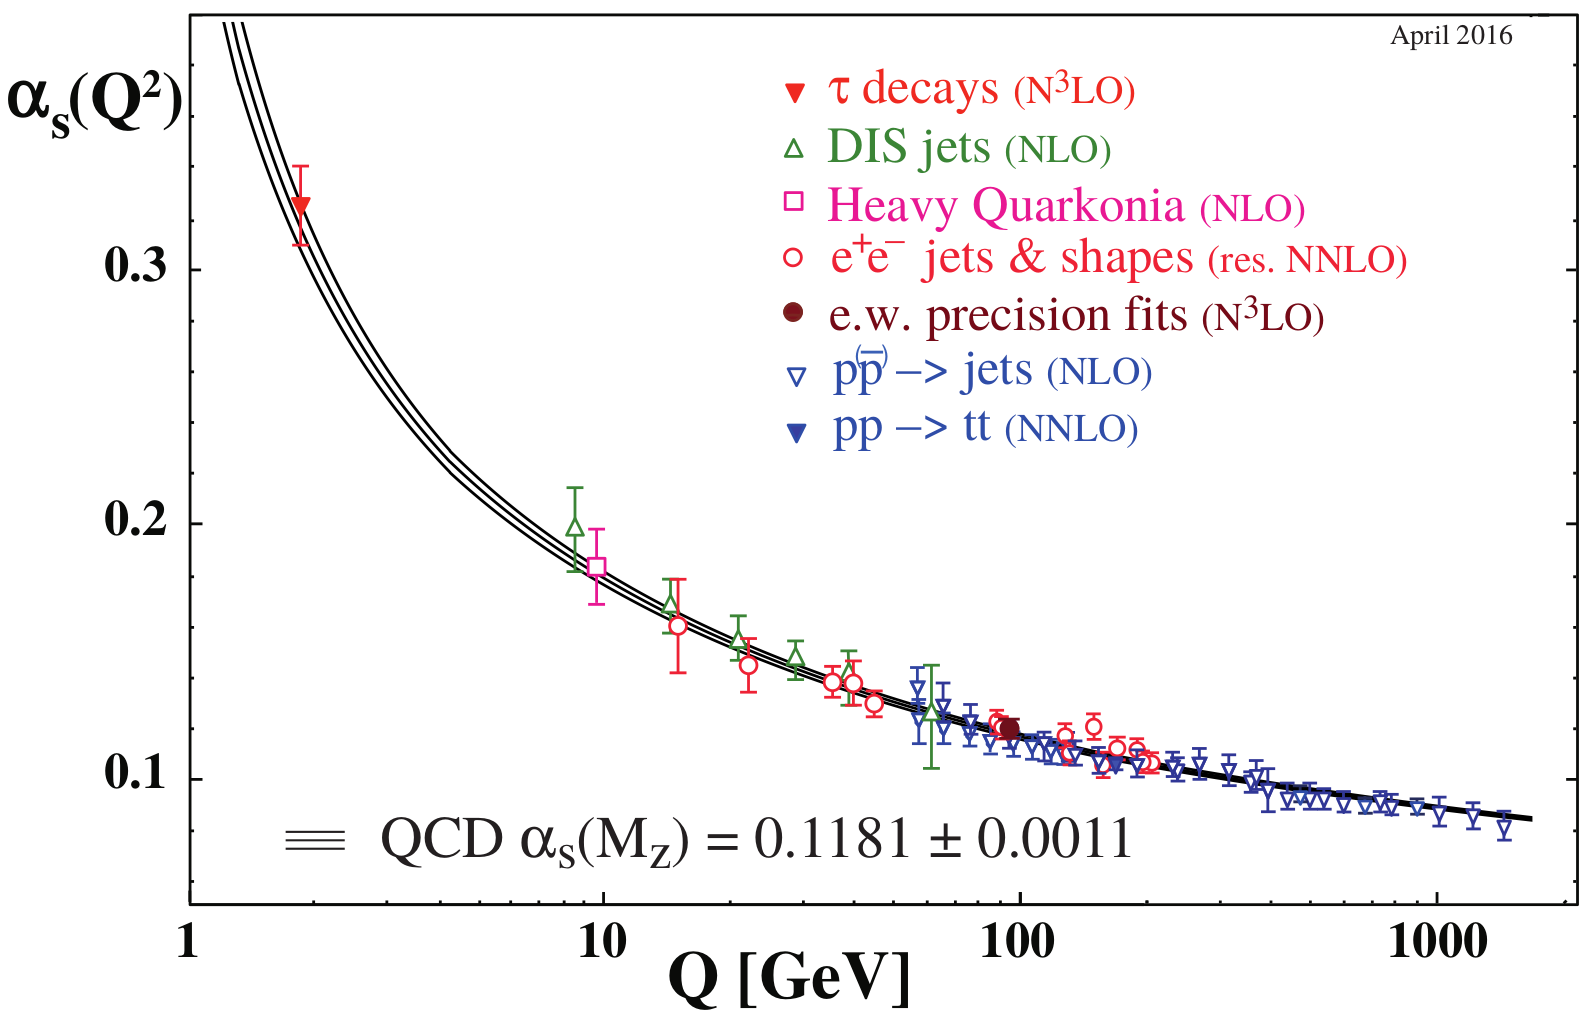
\includegraphics[width=0.6\textwidth]{Figures/Introduction/StandardModel/Alphas.png}
 \caption{Summary of measurements of $\alpha_{s}$ as a function of the energy scale $Q$. Figure taken from the PDG~\cite{PDG}}
 \label{fig:Alphas}
\end{figure}

\subsubsection{Asymptotic freedom}

One important consequence of the non-abelian nature of QCD is the asymptotic freedom of colour charged particles discovered in 1973 by David Gross and Frank Wilczek~\cite{AsymptoticFreedom_1}, and also by David Politzer~\cite{AsymptoticFreedom_2}. As can be observe in \fig{fig:Alphas}, the strength of the strong nuclear force gets asymptotically reduced as the energy scale is increased. Perturbative QCD can then be fully applied in the asymptotic free regime since the strong coupling constant is small.

Considering the inverse relation between the wavelength of particles and their momentum (the de Broglie hypothesis~\cite{Broglie}), asymptotic freedom implies that the strong nuclear interactions between quarks gets weaker at larger momentum or at shorter distances. This phenomenon can be understood qualitatively as derived from the interaction with the QCD vacuum. The presence of virtual quark-antiquark pairs from the vacuum acts as colour dipoles reducing (screening) the strength of the colour charge field. In addition, virtual gluons can couple to other gluons increasing (anti-screening) the net effect of the colour charge seen at larger distances. Thus, there is an interplay between quark-antiquark colour screening and gluon colour anti-screening, where the later effect dominates in QCD.

\subsubsection{Colour confinement}

The fact that quarks and gluons have never been observed isolated in normal conditions is due to another phenomenon of QCD called colour confinement. The intensity of the strong nuclear force increases when the energy scale is reduced or the distance is increased as seen in \fig{fig:Alphas}. The large strong interactions between colour charged particles force the quarks and gluons to be confined in hadrons. The divergent behaviour of $\alpha_{s}$ at the Landau pole shown in \eq{eq:QCDCoupling}, is a consequence of the inability of pQCD to describe the low energy regime, which becomes non-perturbative.%An alternative way to study the low energy regime is to use lattice QCD calculations.

The strong nuclear force can be described qualitatively as a string. When a quark and anti-quark gets separated, the gluon string that mediates their strong interaction elongates, increasing the energy. The string eventually breaks when it becomes more energetically favourable to create a light quark-antiquark pair, splitting the original meson into two mesons as shown in \fig{fig:QCDConfinement}. This leads to a process called hadronisation where quarks and gluons produce a cascade of hadrons. The presence of colour charged particles in high energy collisions can be measured experimentally using jets derived by clustering the final state hadrons in narrow cones.

\begin{figure}[!htb]
 \centering
 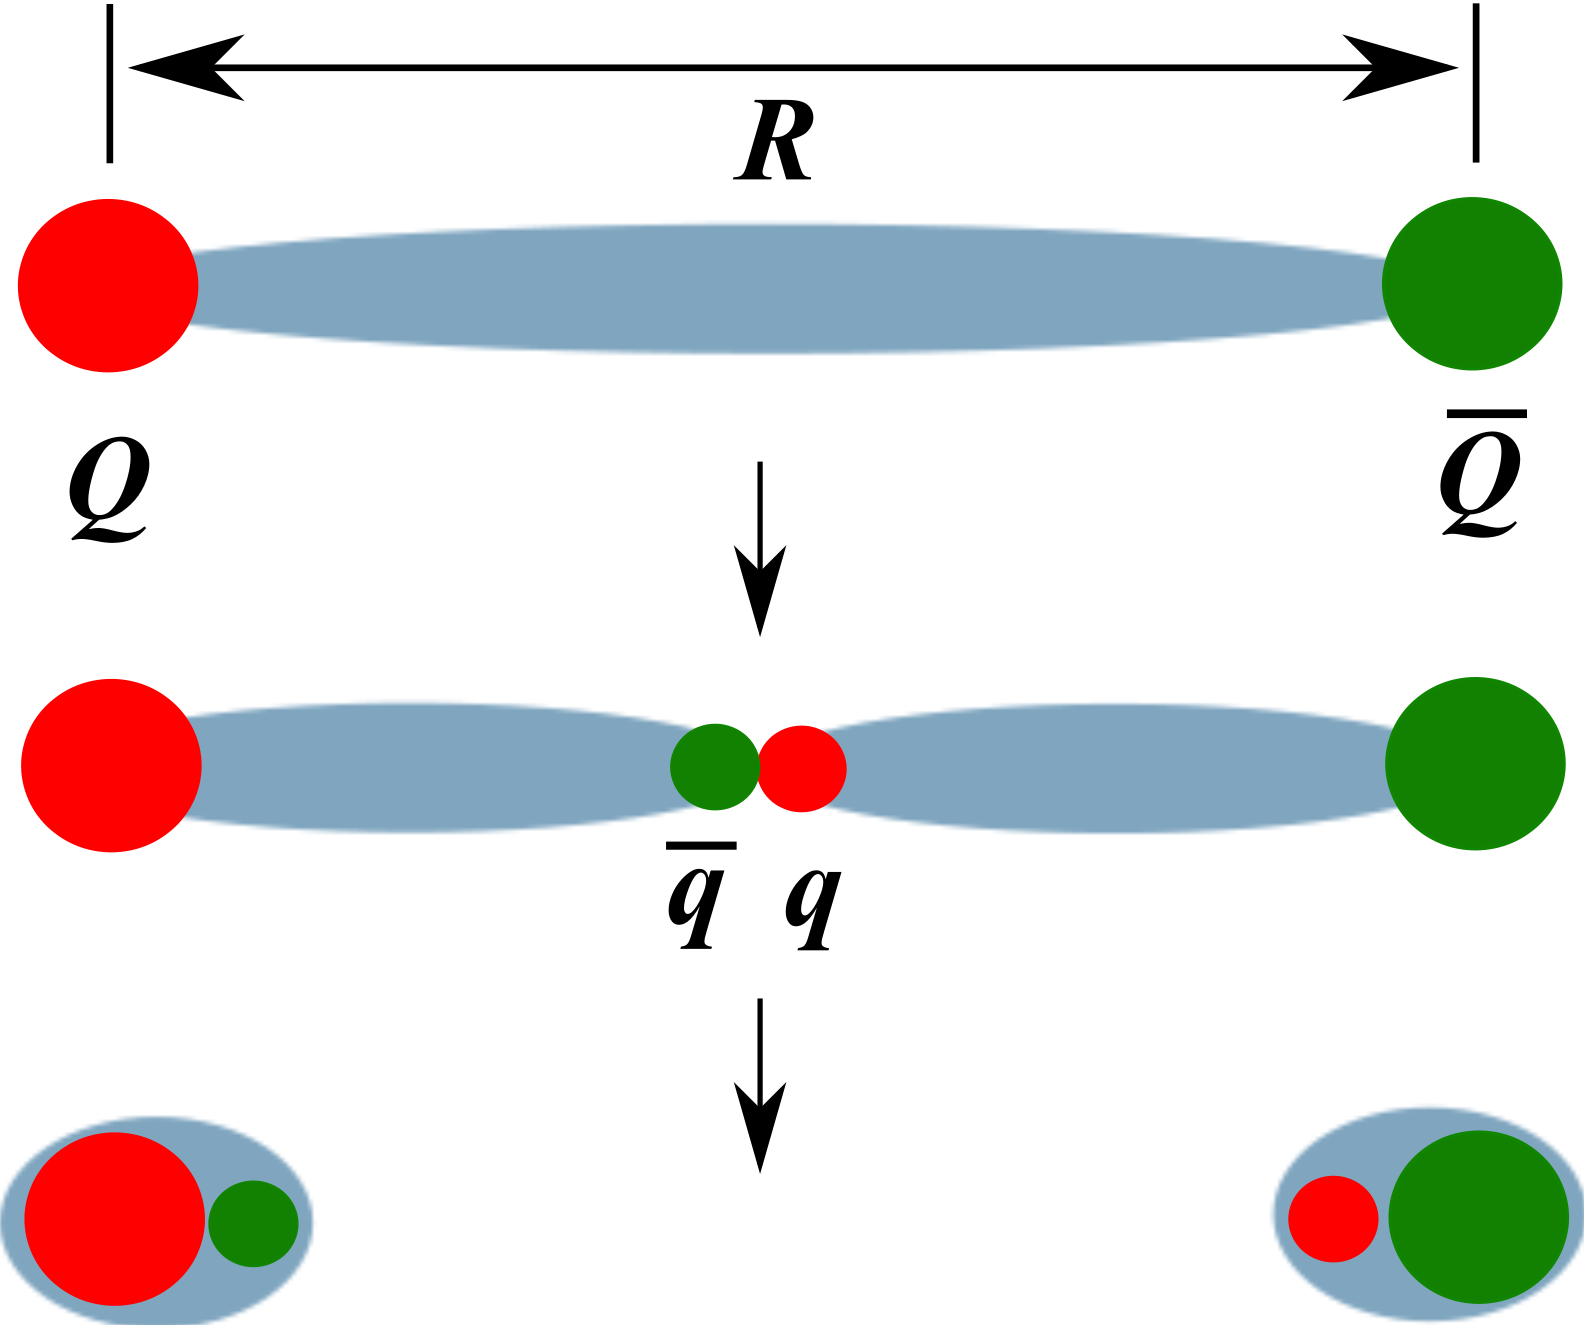
\includegraphics[width=0.3\textwidth]{Figures/Introduction/StandardModel/QCDConfinement.png}
 \caption{Sketch of the gluon string breaking between a quark $Q$ and an anti-quark $\bar{Q}$ due to $q\bar{q}$ pair creation. Figure taken from Ref.~\cite{QCDConfinement_Figure}.}
 \label{fig:QCDConfinement}
\end{figure}

\subsection{Parton distribution functions}\label{sec:Physics_SI_PDF}

The production of particles in hadronic collisions depends on the evolution of the partons (i.e. quarks and gluons) inside the hadrons and the parton momentum transfer during the hard scattering. Since the strong coupling constant decreases with increasing momentum scales, partons can be considered asymptotically free within the hadron during collisions involving large momentum transfer. In this case, each parton carries a fraction of the total momentum of the hadron, represented by the quantity called Bjorken $x$~\cite{BjorkenX} (labelled simply as $x$), given by:

\begin{equation}
p_{parton} = xp_{proton}
\end{equation}

The net quantum properties of hadrons, such as the electric or colour charge, are derived from the valence quarks. The interaction between valence quarks is mediated by the exchange of gluons. Gluons can also produce virtual quark-antiquark pairs and other gluons through self interactions. The virtual quarks produced inside the hadrons are called sea quarks. The gluons and sea quarks do not contribute to the net quantum numbers of the hadron but they can contribute to its mass and they also play a key role in the interaction of hadrons with other particles.

A convenient way of studying the partonic content of hadrons is through the parton distribution functions. The PDF of a hadron represents the probability that a parton carries a given fraction $x$ of the total momentum of the hadron.

According to the QCD factorisation theorem~\cite{QCDFactTheo}, the cross section of a given hard scattering process in hadronic collisions can be split in a partonic cross section times the PDFs of each incoming hadron. On one hand, the partonic cross section can be derived using perturbative QCD and does not depend on the colliding hadrons. On the other hand, the  PDFs can not be calculated from first principles due to the non-perturbative nature of QCD, but they can be determined from global fits to experimental data since the PDFs are independent of the initial scattering process (i.e. universal). The hadronic cross section in a given final state can be expressed at LO, using the factorisation theorem, as:

\begin{equation}
\sigma_{h_{1},h_{2}} = \sum_{f_{1},f_{2}=(\cPq,\cPaq,\cPg)}\int_{0}^{1}\dd{x}_{1}\dd{x}_{2}f_{1}^{h_{1}}\left(x_{1},Q^{2}\right)f_{2}^{h_{2}}\left(x_{2},Q^{2}\right)\hat{\sigma}_{f_{1}f_{2}}
\label{eq:FactTheorem}
\end{equation}

where $Q^{2}$ is the momentum scale, $f^{h_{1}}\left(x,Q^{2}\right)$ is the PDF of a given incoming hadron $h_{1}$, and $\hat{\sigma}_{f_{1}f_{2}}$ represents the partonic cross section of the scattering process between partons $f_{1}$ and $f_{2}$.

The $Q^{2}$ dependence of the PDFs is described by the parton evolution equations developed by Dokshiftzer, Gribov, Lipatov, Altarelli and Parisi (DGLAP)~\cite{DGLAP_1,DGLAP_2,DGLAP_3}. In the DGLAP formalism, the PDFs can be expressed in terms of kernels $P_{q_{1}q_{2}}$ (called splitting functions), and the evolution equations of the parton densities can be written as:

\begin{equation}
  \begin{alignedat}{1}
    \frac{d}{dt}\cPq_{i}\left(x,t\right) &= \frac{\alpha_{s}\left(Q\right)}{2\pi}\left[\cPq_{i}\circledast{P_{\cPq\cPq}} + \cPg\circledast{P_{\cPq\cPg}}\right] \\
    \frac{d}{dt}\cPg\left(x,t\right) &= \frac{\alpha_{s}\left(Q\right)}{2\pi}\left[\sum_{i}\left(\cPq_{i}+\cPaq_{i}\right)\circledast{P_{\cPg\cPq}} + \cPg\circledast{P_{\cPg\cPg}}\right] \\
    \left[q\circledast{P}\right] &= \int_{x}^{1}\dd{y}\frac{q\left(y,t\right)}{y}\times{P\left(\frac{x}{y}\right)}
  \end{alignedat}
  \label{eq:DGLAP}
\end{equation}

where $t = \log\left(Q^{2}/\mu^{2}_{F}\right)$, $\mu_{F}$ is the factorisation scale (energy scale that separates the PDFs from the partonic cross sections), and $P_{q_{1}q_{2}}$ represents the probability that a parton of type $q_{1}$ emits a parton of type $q_{2}$. In other words, the DGLAP evolution equations state that the PDF of a given parton $q$ at an $x$ value is determined from the contribution of all the partons at higher momentum fraction considering their probability of decaying into the parton $q$.

From the definition of the PDFs, one can also formulate a set of structure functions defined as:

\begin{equation}
F^{p}_{2}\left(x\right) = \sum_{q}e_{q}^{2}f\left(x,Q^{2}\right)x
\end{equation}

where $e_{q}$ is the electric charge of a given quark flavour $q$. The structure functions were extensively measured in deep-inelastic scattering (DIS) collisions at the Hadron-Elektron-Ring-Anlage (HERA) accelarator. The DIS process consists in the inelastic scattering of electrons off protons as presented in \fig{dia:DIS}. In the DIS process, the momentum transferred from the electron to the proton is defined as $Q^{2} = -q^{2} = -\left(k - k'\right)^{2}$ and the corresponding Bjorken x fraction is $x = {Q^{2}}\big/{\left(2p{\cdot}q\right)}$, where all 4-momenta are defined in the figure.

\begin{figure}[!htb]
  \vspace{10mm}
  \centering
  \begin{fmffile}{DIS}
    \begin{fmfgraph*}(160,100)
      \fmfleft{ip,il}
      \fmfright{x1,x2,x3,o1,o2,o3,o4,ol}
      \fmfset{arrow_len}{10}
      % lepton
      \fmflabel{$\text{e}^-$}{il}
      \fmflabel{$\text{e}^-$}{ol}
      \fmf{fermion,label=$k$, label.side=left}{il,vl}
      \fmf{fermion,label=$k'$,label.side=left}{vl,ol}
      \fmf{phantom,tension=0.6}{vl,vp}
      % proton
      \fmfv{l=$\text{p}^+$,l.a=-160}{ip} % l.a = label.angle
      \fmf{phantom,tension=1}{ip,vp,x1}
      \fmffreeze
      \fmfi{fermion}{vpath (__ip,__vp) scaled 1.01}
      \fmfi{fermion,label=$p$,label.side=left}
                    {vpath (__ip,__vp) scaled 1.01 shifted (-1.4, 6)}
      \fmfi{fermion}{vpath (__ip,__vp) scaled 1.01 shifted ( 1.4,-6)}
      \fmfblob{25}{vp}
      % X
      \fmfv{l=\mybrace{40} $X$,l.a=10}{x2}
      \fmf{fermion}{vp,x1}
      \fmf{phantom}{vp,x2} % to help \fmfi
      \fmfi{fermion}{vpath (__vp,__x2) scaled 0.98 shifted (0,2.2)}
      \fmffreeze
      % photon
      \fmf{photon,label=\vspace{-4pt}\hspace{5pt}{$q$},label.side=left}{vl,v}
      % parton
      \fmf{fermion,label=$xp$,label.side=left}{vp,v}
      \fmf{fermion}{v,o2}
    \end{fmfgraph*}
  \end{fmffile}
  \caption{Feynman diagram of deep inelastic scattering of electrons against protons.}
  \label{dia:DIS}
\end{figure}

The measurements of the $F_{2}$ structure function performed by the ZEUS collaboration~\cite{HERAStrucFunc} at HERA are shown in \fig{fig:HERAStrucFunc}. Even though DIS experiments were not able to probe the gluons directly, the DIS data showed that valence quarks only carry half of the proton momentum, the other half being carried by the gluons.

\begin{figure}[!htb]
 \centering
 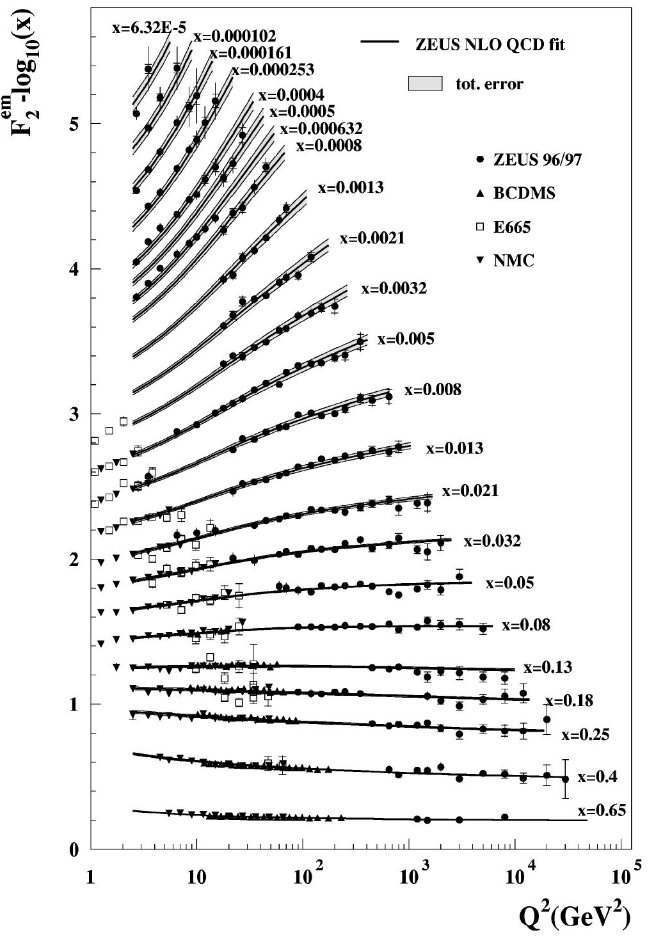
\includegraphics[width=0.4\textwidth]{Figures/Introduction/StandardModel/Structure_Function.png}
 \caption{Next-to-leading order QCD fits to the to the ZEUS $F_{2}$ structure function data from 1996, 1997 and proton fixed-target at HERA. The error bands of the fit represent the total experimental uncertainty from both correlated and uncorrelated sources. Figure taken from Ref.~\cite{HERAStrucFunc}.}
 \label{fig:HERAStrucFunc}
\end{figure}

Another important process used to constrain PDFs is the Drell-Yan (DY) process or the production of \Wb bosons. In the DY process, a quark from one hadron and an anti-quark from another hadron annihilate into a virtual photon ($\gamma^{*}$) or a \Z boson, which then decays to a particle-antiparticle pair as shown in \fig{dia:DY}. The measurement of DY production can be used to constrain the quark PDFs in a wide range of momentum fraction x depending on the invariant mass of the dilepton pair. In addition, the measurement of the production of positive and negative charged \Wb bosons in hadronic collisions is used to disentangle the flavour dependence of the quark PDFs. More details about the \Wb boson production will be provided in \chp{sec:WBoson}, since the present thesis report a measurement of \Wb bosons in \RunpPb collisions that provide strong constraints on nuclear PDF.

\begin{figure}[!htb]
  \vspace{10mm}
  \centering
  \begin{fmffile}{DY}
  \begin{fmfgraph*}(160,160)
    \fmfleft{i1,iq,i2,ip,i3}
    \fmfright{y1,y2,y3,o1,f1,o2,o3,o4,f2,o5,x3,x2,x1}
    \fmfset{arrow_len}{10}
    % skeleton
    \fmf{phantom,tension=0.48}{vq,vp}
    \fmf{phantom}{ip,vp,x1}
    \fmf{phantom}{iq,vq,y1}
    \fmffreeze
    % parton
    \fmfv{l=$x_1p_1$,l.a=-90,l.d=22}{vp} % cheat: actually a line label
    \fmfv{l=$x_2p_2$,l.a=90,l.d=22}{vq} % cheat: actually a line label
    \fmf{fermion,tension=1.6}{vp,v}
    \fmf{fermion,tension=1.6}{v,vq}
    % hard process
    \fmfshift{20 right}{f1,f2}
    \fmfv{l=$\bar{f}$}{f1}
    \fmfv{l=$f$}{f2}
    \fmf{boson,tension=2,label=$\text{Z}^0/\gamma^*$,label.side=left}{v,vf}
    \fmf{fermion,tension=2}{f1,vf,f2}
    % proton 1
    \fmfv{l=${h}_{A}$,l.a=180,l.d=10}{ip}
    \fmf{phantom}{ip,vp}
    \fmfi{fermion,l=$p_1$,l.s=left,l.d=8}
                  {vpath (__ip,__vp) scaled 1.01 shifted (-2.4, 6)}
    \fmfi{fermion}{vpath (__ip,__vp) scaled 1.01 shifted (-2.4, 0)}
    \fmfi{fermion}{vpath (__ip,__vp) scaled 1.01 shifted (-2.4,-6)}
    % proton 2
    \fmfv{l=${h}_{B}$,l.a=180,l.d=10}{iq}
    \fmf{phantom}{iq,vq}
    \fmfi{fermion}{vpath (__iq,__vq) scaled 1.01 shifted (-2.4, 6)}
    \fmfi{fermion}{vpath (__iq,__vq) scaled 1.01 shifted (-2.4, 0)}
    \fmfi{fermion,l=$p_2$,l.s=right,l.d=8}
                  {vpath (__iq,__vq) scaled 1.01 shifted (-2.4,-6)}
    % X 2
    \fmfshift{25 left}{x1}
    \fmfshift{20 left}{x2,x3}
    \fmf{phantom}{vp,x1} % to help \fmfi
    \fmf{phantom}{vp,x2} % to help \fmfi
    \fmf{phantom}{vp,x3} % to help \fmfi
    \fmfi{fermion}{vpath (__vp,__x1) scaled 1.0 shifted ( 0.0, 2.0)}
    \fmfi{fermion}{vpath (__vp,__x2) scaled 1.0 shifted ( 0.0, 0.0)}
    \fmfi{fermion}{vpath (__vp,__x3) scaled 1.0 shifted ( 0.0,-2.0)}
    \fmfblob{25}{vp}
    % X 2
    \fmfshift{25 left}{y1}
    \fmfshift{20 left}{y2,y3}
    \fmf{phantom}{vq,y1} % to help \fmfi
    \fmf{phantom}{vq,y2} % to help \fmfi
    \fmf{phantom}{vq,y3} % to help \fmfi
    \fmfi{fermion}{vpath (__vq,__y1) scaled 1.0 shifted ( 0.0,-2.0)}
    \fmfi{fermion}{vpath (__vq,__y2) scaled 1.0 shifted ( 0.0, 0.0)}
    \fmfi{fermion}{vpath (__vq,__y3) scaled 1.0 shifted ( 0.0, 2.0)}
    \fmfblob{25}{vq}
  \end{fmfgraph*}
  \end{fmffile}
  \caption{Feynman diagram of the Drell-Yan process.}
  \label{dia:DY}
\end{figure}

\subsection{QCD phase diagram}\label{sec:Physics_SI_PhaseDiagram}

The first attempt to describe the temperature evolution of matter at high energies was performed by Rofl Hagedorn in 1965~\cite{Hagedorn1965}. Hagedorn considered matter at high energies as a gas made of hadrons and he employed a thermodynamical bootstrap approach to describe the hadron gas. After studying the mass spectrum of all the hadron species measured at the time, Hagedorn realised that the density of hadron species grows exponentially until it diverges at a temperature of $T_{H} \approx 158$~MeV, known as the Hagedorn temperature. Years later, with the advent of QCD, it was understood that the Hagedorn temperature described a transition from a hadron gas to a state of matter where quarks and gluons are asymptotically free called the quark-gluon plasma.

The description of the QCD phase transition turned out to be complicated because the critical temperature is close to the QCD scale $\Lambda_{\text{QCD}} \approx \SI{255}{\MeV}$~\cite{LambdaQCD}, where perturbative calculations are no longer reliable. An alternative method to study the non-perturbative regime of QCD consists of solving numerically the QCD field equations on a discrete space-time grid using a method called lattice QCD. Nowadays, lattice QCD is able to describe the evolution of matter at finite temperatures and low densities. A sketch of the QCD phase diagram in terms of the temperature $T$ and the baryon chemical potential $\mu_{\B}$\footnote{The baryon chemical potential can be viewed as a measure of the excess of matter over anti-matter and it is proportional to the baryon density.}. is shown in \fig{fig:QCDPhaseDiagram}.

\begin{figure}[!htb]
 \centering
 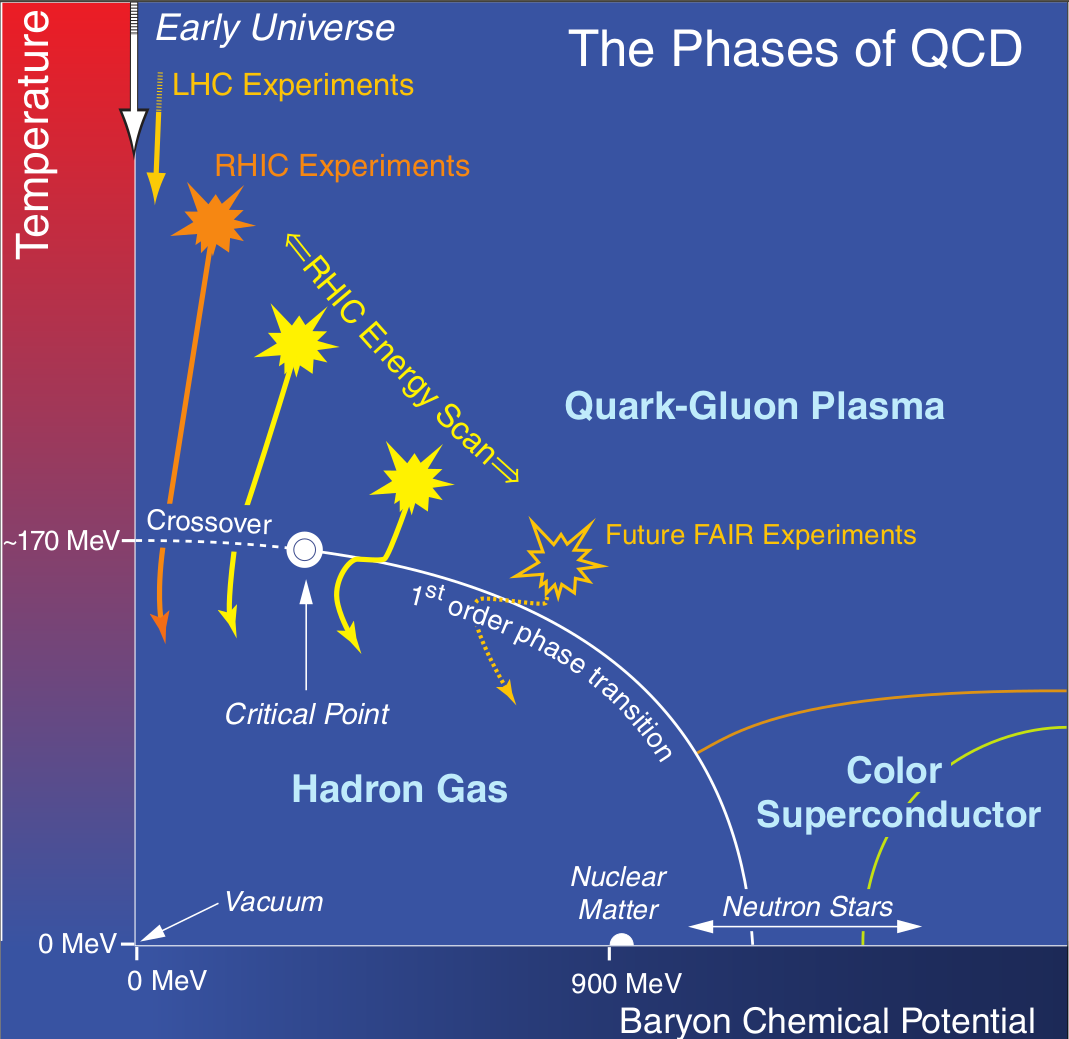
\includegraphics[width=0.6\textwidth]{Figures/Introduction/StandardModel/QCDPhaseDiagram.png}
 \caption{Sketch of the QCD phase diagram for nuclear matter. The solid lines show the phase boundaries and the solid circle represents the critical point. Figure taken from Ref.~\cite{QCDPhaseDiagram}.}
 \label{fig:QCDPhaseDiagram}
\end{figure}

Normal nuclear matter exists in nature at low temperatures and high $\mu_{\B}$ (\SI{900}{\MeV}). At higher $\mu_{\B}$, matter undergoes a phase transition to a degenerate gas of fermions, known as neutron gas, which is present in neutron stars. It is theorised that at even higher $\mu_{\B}$, matter could reach a state of colour superconductivity where quarks bind together into Cooper pairs~\cite{ColorSupercondutor}. On the other hand, matter present at the beginning of the universe or produced in TeV-scale particle collisions has very low baryon chemical potential. Matter is described at low temperatures as a hadron gas and it becomes a QGP when the temperature exceeds some critical value. At low $\mu_{\B}$, the phase transition between the hadron gas and the QGP has been established, using lattice QCD, to be a crossover where the two states coexist~\cite{LatticeQCD,LatticeQCD2}.


\section{Relativistic heavy-ion collisions}\label{sec:Physics_HI}

Heavy-ion colliders have become essential tools to explore the fundamental properties of matter. Collisions of nuclei are used to probe the phase transitions of QCD and to recreate the QGP in the laboratory. The QGP is believed to have existed at the beginning of the Universe and to be part of the core of some astrophysical objects such as neutron stars. The study of the QGP allows to test QCD in the most extreme regimes and provides an insight on the evolution of the Universe. Some of the primary research goals of the heavy-ion physics programme is to understand the formation and properties of the QGP, and how does matter interact with the nuclear medium. Nowadays, the experimental study of ultra-relativistic (i.e. at energies above $\sqrtsnn > \SI{10}{\GeV}$) heavy-ion collisions is performed at the Brookhaven National Laboratory (BNL) and at the European Organization for Nuclear Research (CERN).


\subsection{History of heavy-ion accelerators}

The interest in probing the QCD phase diagram in the laboratory arose in the 1970s after Werner Scheid, Hans M{\"u}ller and Walter Greiner predicted that nuclear matter could be compressed in heavy-ion collisions at nucleus-nucleus energies larger than 100~\si{\MeV}/nucleon~\cite{MatterShock}. The shock compression mechanism could reach matter densities up to five times higher than the density of atomic nuclei ($\rho_{0}=0.16~baryons/\si{\femto\meter\cubed}$)~\cite{MatterShock}. Coinciding in time, the Lawrence Berkeley National Laboratory (LBNL) decided to transform their proton synchrotron accelerator Bevatron into a heavy-ion experiment called Bevalac. Heavy ions were produced in the Bevalac using the heavy-ion linear accelarator SuperHILAC and then sent to the Bevatron, where the ions were further accelerated against a fixed target with energies of up to \SI{2.6}{\GeV}/nucleon~\cite{Bevalac}. The goal at the time was to investigate the equation of state (EoS) of hadronic matter at high densities. The understanding of the relation between the pressure and the energy density of dense matter was a key element needed to describe the dynamics of astrophysical objects such as neutron stars~\cite{NeutronStar, DenseMatter}.

The successful creation of compressed nuclear matter at the Bevatron motivated the construction of several heavy-ion accelerators at higher energies. The first one was the Alternating Gradient Synchrotron (AGS) particle accelerator at the Brookhaven National Laboratory (BNL). The AGS became the first facility in 1960 to accelerate protons to an energy of \SI{33}{\GeV}, which allowed to discover the muon neutrino in 1962 and to observe the CP violation of the weak interactions in Kaon decays in 1964. An electrostatic accelerator called the Tandem Van de Graaf was built in 1970 to provide beams of ions to the AGS. The relativistic heavy-ion programme started at AGS in 1986 and lasted for 12 years during which several experiments were performed (e.g. E802, E858, E866, E896 and E917). The AGS accelerated Si beams at \SI{14.6}{\GeV}/nucleon and Au beams at \SI{11.1}{\GeV}/nucleon, and collided them against different types of fixed targets (e.g. Al and Au).

In parallel, CERN built the Super Proton Synchroton (SPS) in 1976. To study the QGP, CERN added an Electron-Cyclotron Resonance (ERC) ion source in 1986 which initially accelerated ions of oxygen and sulphur at \SI{200}{\GeV}/nucleon. A subsequent upgrade of the ion injector in 1994 allowed to accelerate up to an energy of \SI{158}{\GeV}/nucleon the Pb ions, which were collided against fixed targets located in two experimental halls: one in the SPS north area (NA) and the other in the SPS west area (WA). Several fixed target experiments were built at the SPS between 1986 and 2005. After years of analysing the Pb-Pb and Pb-Au fixed target collision data from SPS, CERN announced in 2000 that the combined results of the experiments NA44, NA45, NA49, NA50, NA52, WA97/NA57 and WA98, provided a first evidence of the creation of a new state of matter consistent with the QGP~\cite{SPSQGP}.

In the meantime, the first nucleus-nucleus collider, known as the Relativistic Heavy Ion Collider (RHIC), started operations at the BNL in 2000. Two beams of Au are pre-accelerated at the AGS to an energy of \SI{8.86}{\GeV}/nucleon and then sent to RHIC where the Au beams were first collided at $\sqrtsnn = \SI{130}{\GeV}$, and later at \SI{200}{\GeV}. Other collision systems explored at RHIC include: p-p, p-Au, d-Au, Cu-Cu, Cu-Au and U-U~\cite{RHICRuns}. There were four detectors at RHIC called BRAHMS, PHENIX, STAR, and PHOBOS. Currently, only the STAR and PHENIX collaborations are still active, while PHOBOS ceased operations in 2005 and BRAHMS in 2006. After four years of meticulously studying the system produced in Au-Au collisions with the four detectors, RHIC finally announced in 2005 the discovery of a strongly coupled QGP. Contrary to the expected gaseous behaviour, the QGP observed at RHIC turned out to resemble more a liquid with very little viscosity~\cite{BRAHMS_QGP,PHENIX_QGP,STAR_QGP,PHOBOS_QGP}.

Currently, the largest heavy-ion collider is the Large Hadron Collider (LHC) at CERN, whose construction finished in 2008. The SPS is used as injector to the LHC, accelerating the Pb beams to energies of \SI{1.38}{\TeV}. The first nucleus-nucleus collisions at LHC took place in 2010 using Pb beams at \SI{2.76}{\TeV}. Since then, the LHC has collided different configurations involving ions, including p-Pb at \SI{2.76}{\TeV} (2013), Pb-Pb at 5.02~TeV (2015), p-Pb at \SI{8.16}{\TeV} (2016), Xe-Xe at \SI{5.44}{\TeV} (2017), and at the end of 2018 LHC is planning to provide a larger set of Pb-Pb collisions at \SI{5.02}{\TeV}. There are four detectors at the LHC called ALICE, CMS, ATLAS and LHCb. The four experiments are nowadays participating in the heavy-ion programme at LHC. Due to the large beam energies, the LHC is an ideal collider to study the QGP at very high temperatures, where one expects smaller QGP formation times and larger hot medium densities, compared to RHIC.


\subsection{Geometry of nucleus-nucleus collisions}\label{sec:Physics_HI_Glauber}

The number of particles produced in a nucleus-nucleus collision depends on the geometry of the collision. Since nuclei are extended objects made of nucleons (i.e. protons and neutrons), the number of nucleon-nucleon (NN) interactions increases the more head-on or central is the collision. The nucleons that participate in the collision are called participants while those that do not participate are referred to as spectators. The overlap region of the collision depends on the impact parameter $\vec{b}$, which is the transverse distance between the centres of the two colliding nuclei as shown in \fig{fig:CollisionGeometry}.

\begin{figure}[!htb]
 \centering
 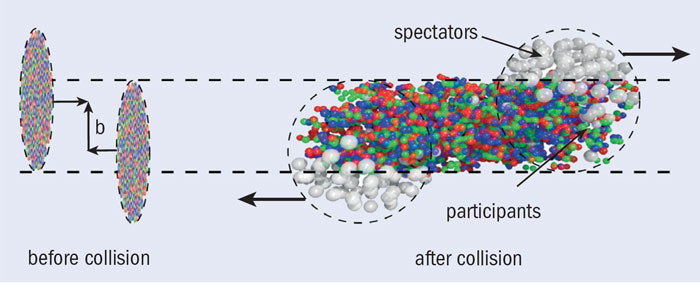
\includegraphics[width=0.9\textwidth]{Figures/Introduction/HeavyIons/CollisionGeometry.jpg}
 \caption{Illustration of two nucleus with impact parameter b before (left) and after (right) colliding. Figure taken from Ref.~\cite{QCDPhaseDiagram}.}
 \label{fig:CollisionGeometry}
\end{figure}

The formation and characteristics of the QGP in nucleus-nucleus collisions depends on the number of colliding nucleons. To study the dynamics of the nuclear medium, the heavy-ion collisions are classified based on their centrality. The centrality $c$ is defined as the fraction of the total nucleus-nucleus inelastic cross section $\sigma^{\text{inel}}_{\text{AB}}$ determined within the area defined by the impact parameter $b$, and it is  expressed as:

\begin{equation}
 c = \frac{{\pi}b^{2}}{\sigma^{\text{inel}}_{\text{AB}}}
\end{equation}

The collision centrality can be related to the number of participants \npart and the number of binary nucleon-nucleon collisions \ncoll using a Glauber model. The Glauber model, developed in the 1950s by Roy Glauber, describes the collision between two nuclei as a superposition of independent NN interactions~\cite{GlauberModel}.

There are two ways of implementing the Glauber model, the optical and the Monte Carlo approaches. In the optical approach, the physical observables are computed using the optical limit which assumes a continuous nucleon density distribution. On the other hand, in the Monte Carlo approach, the two nuclei are simulated by distributing the nucleons according to their nuclear density profile, and then the nucleus-nucleus collisions are modelled, at random impact parameters, by computing the individual NN collisions~\cite{GlauberModel}.

An example of a heavy-ion collision described by the optical Glauber model geometry is shown in \fig{fig:GlauberModel}. It represents the collision between a nucleus A with A nucleons and a nucleus B with B nucleons.

\begin{figure}[!htb]
 \centering
 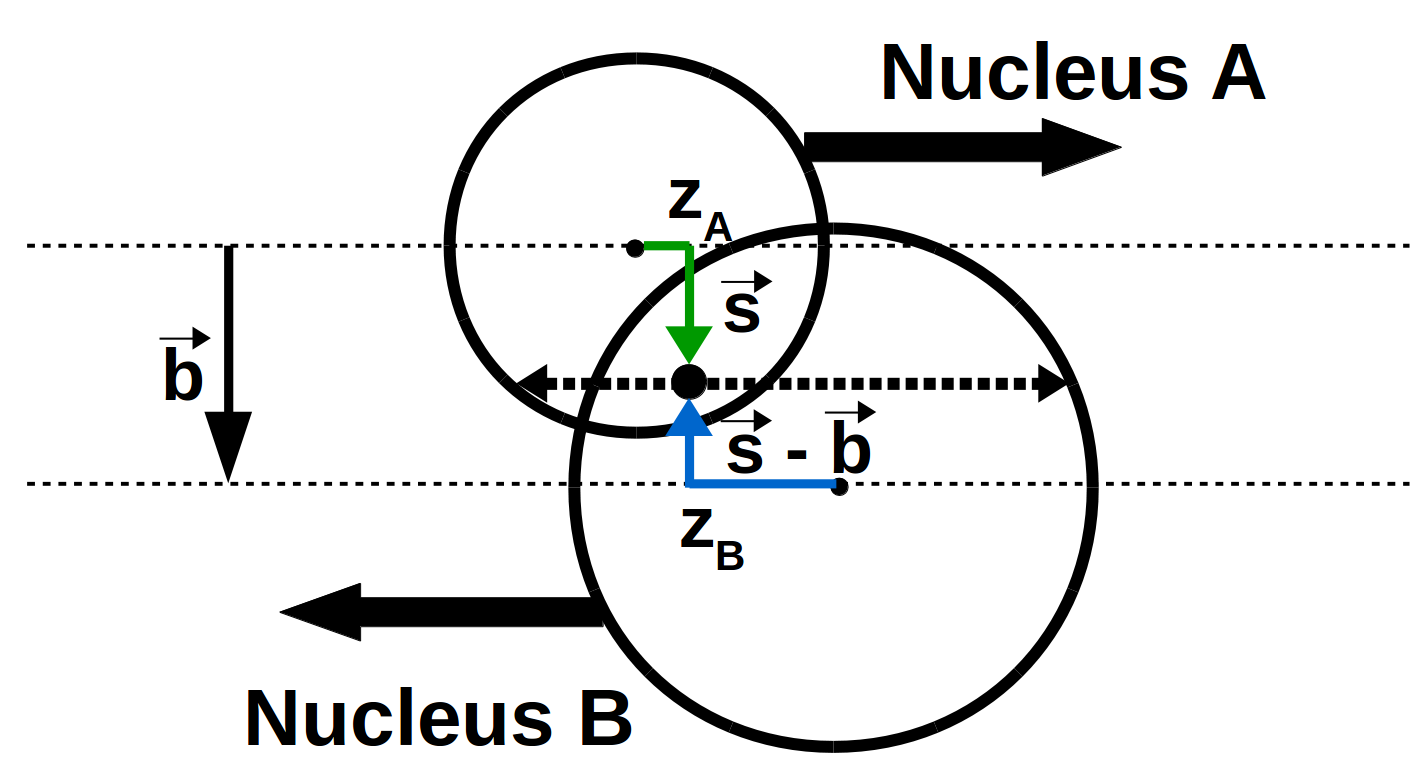
\includegraphics[width=0.7\textwidth]{Figures/Introduction/HeavyIons/GlauberModel.png}
 \caption{Schematic representation of the optical Glauber model geometry.}
 \label{fig:GlauberModel}
\end{figure}

The tube located at a distance $\vec{s}$ from the center of the nucleus A overlaps the tube located at a distance $\vec{b} - \vec{s}$ from the center of the nucleus B. In this case, the nuclear overlap function $T_{\text{AB}}\left(b\right)$ is defined as:

\begin{equation}
  T_{\text{AB}}\left(b\right) = {\int}{\dd{s}^{2}}T_{\text{A}}\left(\vec{s}\right)T_{\text{B}}\left(\vec{b}-\vec{\text{s}}\right)
\end{equation}

where $T_{\text{A}}$ and $T_{\text{B}}$ are the nuclear thickness functions of the nucleus A and B, respectively.

The nuclear thickness function is given by $T\left(\vec{r}\right) = {\int}{\dd{z}}{\rho}\left(\vec{r},z\right)$, where $\rho$ is the nuclear density distribution of a given nucleus, which is generally parametrised with a Wood-Saxon density profile~\cite{GlauberModel}:

\begin{equation}
  \rho\left(r\right) = \frac{\rho_{0}}{1+\exp{\left(\frac{r-r_{0}}{a}\right)}}
\end{equation}

where  $r$ is the distance to the center of the nucleus, $a$ represents the width of the edge region of the nucleus called the skin depth, $r_{0}$ is the mean radius of the nucleus and $\rho_{0}$ is the nuclear density at the center of the nucleus. The average number of binary NN collisions $\left\langle\ncoll\right\rangle$ for a given impact parameter b is defined as:

\begin{equation}
\left\langle\ncoll\left(\text{b}\right)\right\rangle = \text{AB} \cdot \left\langle{T_\text{AB}}\left(b\right)\right\rangle \cdot \sigma^{\text{inel}}_{\text{nn}}
\end{equation}

where $\sigma^{\text{inel}}_{\text{nn}}$ is the inelastic nucleon-nucleon cross section and $\left\langle{T_\text{AB}}\left(b\right)\right\rangle$ is the average nuclear overlap function. Hence, the Glauber model provides a quantitative description of the geometry of the nuclear collision and can be used to estimate the variables (\npart, \ncoll and $T_{\text{AB}}$) for a given centrality class.

Experimentally, the impact parameter of the collision can not be determined directly. However, the distribution of the number of soft particles scales with $N_{part}$. As a result, one can classify the events in different  centrality classes by binning the measured distribution of charged particles, so that each bin contain the same fraction of the total integral. The mean parameters $\left\langle\npart\right\rangle$ and $\left\langle\ncoll\right\rangle$, can be then derived, for each centrality class, by simulating the charged-particle distribution using a MC Glauber model. In addition, the collision centrality can sometimes be also inferred from the number of spectators determined from the measurement of the transverse energy in the forward region.


\subsection{Evolution of heavy-ion collisions}

The evolution of a nucleus-nucleus collision undergoes several steps, starting from the collision of the nuclei to the final production of hadrons. Figure~\ref{fig:QGPEvolution} illustrates the different processes that occur during a heavy-ion collision associated to the production of the QGP.

\begin{figure}[!htb]
 \centering
 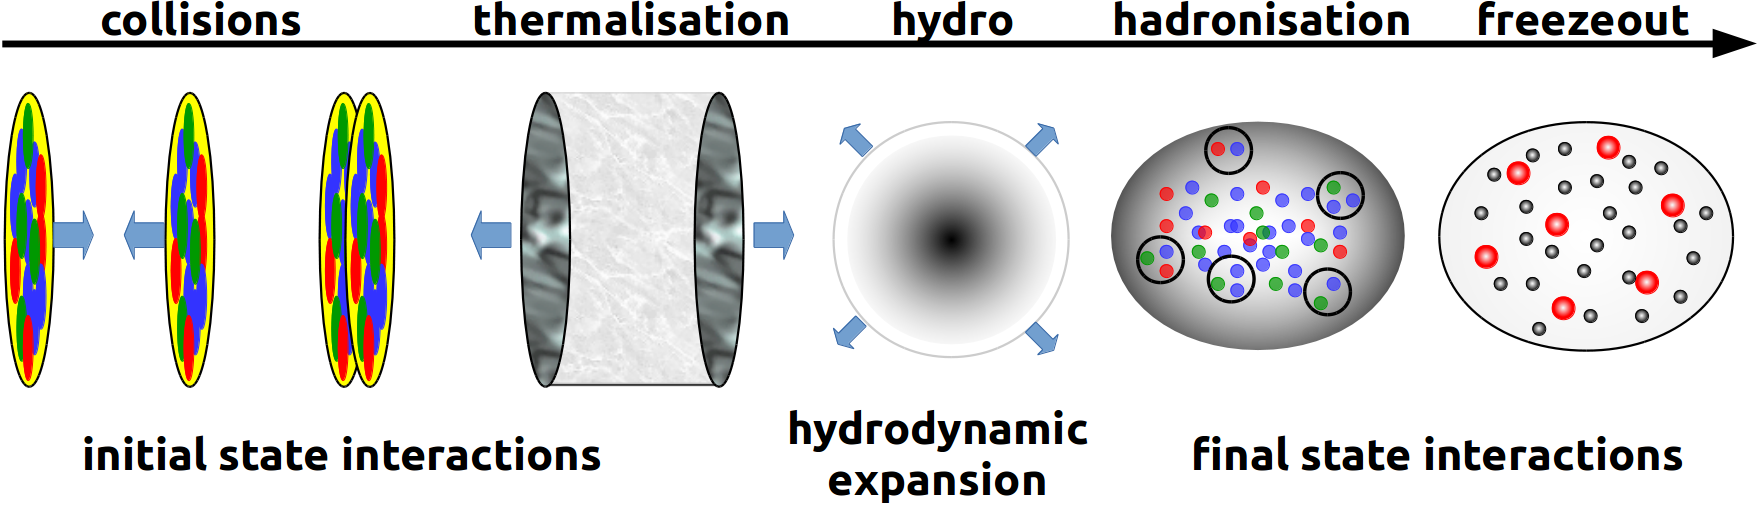
\includegraphics[width=1.0\textwidth]{Figures/Introduction/HeavyIons/QGPEvolution.png}
 \caption{Sketch of the evolution of a relativistic heavy-ion collision.}
 \label{fig:QGPEvolution}
\end{figure}

\begin{enumerate}

\item Initial stage: At high energies, the two nuclei are Lorentz contracted along the axis of motion while approaching each other at almost the speed of light. As a consequence, the nucleons of each nuclei are also contracted increasing the number of gluons until it reaches the gluon saturation scale. The initial conditions can be described in various ways, depending on the physics to be addressed: the Glauber moder or the effective theory called the Color Glass Condesate are often used. When the two nuclei collide, the partons inside the geometrical overlap region of the two nuclei undergo parton-parton interactions.\\

\item QGP formation and thermalisation: The parton-parton interactions quickly start producing new particles increasing the density of the system until a phase transition is reached forming the QGP. After some time, the system reaches thermal equilibrium. \\

\item Hydrodynamical expansion: After reaching the thermal equilibrium, the system evolves as a nearly-perfect fluid. It first expands longitudinally along the beam direction and then it expands in all directions until the QGP cools down back to the critical temperature. \\

\item Hadronisation: The medium undergoes a second phase transition back to a hadronic gas where the partons recombine into hadrons. In this phase, the system keeps expanding via hadron-hadron interactions until the average path length of the hadrons is as large as the size of the system. \\

\item Freeze-out: The hadron gas experience first a chemical freeze-out when the inelastic collisions between hadrons cease, fixing the composition of the particles. Subsequently, the system reaches a kinetic freeze-out when the elastic scattering between the hadrons also stop, fixing the kinematic distributions of the particles. Subsequently, the particles escape the medium and are reconstructed in  the detector.

\end{enumerate}

\subsection{Experimental probes of the QGP}

The QGP can not be directly measured experimentally, since once it is created it only exists for a very short amount of time. Nonetheless, the QGP can be studied indirectly by measuring how the particles and the system produced in the collision are modified by the presence of the QGP. There are many experimental \textit{signatures} that has been used to asses the different properties of the QGP, such as the enhancement of the strange quark production, suppression of the quarkonium yields, attenuation of the energy of jets, anisotropies in the azimuthal distribution of particles, among others. The production mechanism of each experimental probe depends on the momentum scale of the process. Signatures produced in processes involving large momentum transfer are called hard probes while those produced at low momentum scales are called soft probes.

The majority of the particles produced in heavy-ion collisions are soft and constitute the bulk of the system. Soft probes are used to study the thermal and hydrodynamical evolution of the medium. The production yields of soft particles scales with \npart. The strange hadron yields and the elliptic flow are two examples of soft probes. On the other hand, hard probes are produced from the parton-parton hard scattering during the initial stage of the collision. Hard probes are ideal tools to study the structure of the system since they are produced early in a well-controlled manner\footnote{The production cross section of hard probes can be computed using the QCD factorisation theorem.} and often living through the QGP. The number of hard particles produced in the medium  scales with \ncoll. Some important hard probes used to study the nuclear medium includes the electroweak bosons, quarkonia and jets. The following subsections present a brief description on some of the soft and hard probes of the QGP.


\subsubsection{Elliptic flow}

When the QGP is formed, it undergoes a collective expansion due to the large pressure gradient produced by the multiple partonic interactions during the heavy-ion collision. This collective expansion is known as flow. The magnitude of the flow tend to grow with the number of parton-parton interactions and it depends on the initial conditions of the collision. If the nucleus-nucleus collision is completely central ($b = 0$) then the particles develop a radial flow, but if the collision is non-central ($b \neq 0$) then the spacial anisotropy of the overlap region leads to an additional anisotropic flow as shown in \fig{fig:ReactionPlane}.

\begin{figure}[!htb]
 \centering
 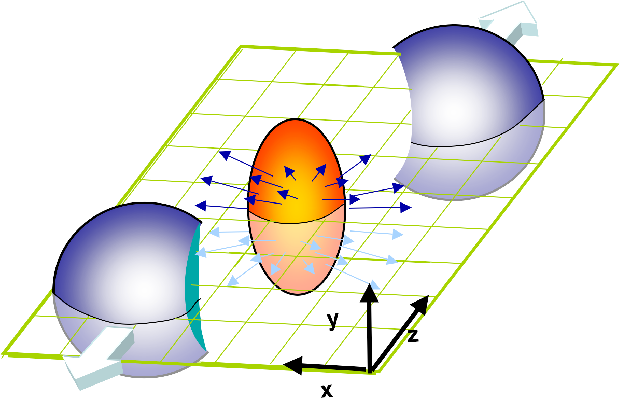
\includegraphics[width=0.6\textwidth]{Figures/Introduction/HeavyIons/ReactionPlane.png}
 \caption{Sketch of the elliptic flow produced in non-central heavy-ion collisions. Figure taken from Ref.~\cite{ReactionPlaneFigure}.}
 \label{fig:ReactionPlane}
\end{figure}

Experimentally, the anisotropic flow can be determined from the Fourier decomposition of the particle azimuthal angle $\phi$ distribution with respect to the reaction plane $\psi_{\text{RP}}$~\cite{EllipticFlowReview}:

\begin{equation}
  \frac{d^{3}N}{d^{3}\vec{p}} = \frac{1}{2\pi}\frac{d^{2}N}{{\pt}{d\pt}{dy}}\left(1 + 2\sum^{\inf}_{n=1}{v_{n}\cos\left[n\left(\phi-\psi_{RP}\right)\right]}\right)
\end{equation}

where the Fourier coefficient $v_{2}$ measures the strength of the elliptic flow and the reaction plane is derived from the direction of the beam ($z$-axis) and the impact parameter ($x$-axis) as presented in \fig{fig:ReactionPlane}.

An alternative way to derive the flow coefficients is by computing the Fourier decomposition of the two-particle azimuthal distribution defined as~\cite{EllipticFlowReview}:

\begin{equation}
  v_{n}\left\{2\right\}^{2} = c_{n}\left\{2\right\} = \left<\cos\left[n\left(\phi_{1} - \phi_{2}\right)\right]\right>
\end{equation}

where $c_{n}\left\{2\right\}$ is called the two-particle cumulant and the brackets represent the average over all particles and events. The advantage of using particle correlations is that the Fourier coefficients do not depend on the reaction plane determination, but non-flow contributions (e.g. resonance decays or back-to-back jets) can affect the measurements. Correlating more than two particles, such as four-particle correlations, can reduce the impact of the non-flow effects.

The elliptic flow of the medium is sensitive to the equation of states of the QGP~\cite{EllipticFlowReview} and bulk viscosity~\cite{EllipticFlowViscosity}. Furthermore, relativistic hydrodynamic calculations~\cite{EllipticFlowReview_2} predicts that the elliptic flow of hadrons can approximately be expressed as $v_{2} \propto \left(\pt - {\beta}{\cdot}m_{\text{T}}\right)$, where $\beta$ is the average flow velocity and $m_{\text{T}}$ is the transverse mass of the hadron, which is defined as $m^{2}_{\text{T}} = m^{2} + \pt^{2}$. As a consequence, the elliptic flow is expected to show a mass ordering where the more massive hadrons would have lower $v_{2}$ values compared to the lighter hadrons.

The low {\pt}-dependence of the elliptic flow of strange hadrons measured at RHIC in Au-Au collisions at $\sqrtsnn = \SI{200}{\GeV}$ is presented in \fig{fig:RHICEllipticFlow}. The measurement of the elliptic flow of $\pi^{\pm}$ mesons, $K^{0}_{s}$ mesons, antiprotons and $\Lambda$ baryons (with masses of 140, 495, 940 and 1,115 MeV, respectively), shows the expected mass ordering pattern. Moreover, the good agreement between the RHIC results and the predictions using relativistic hydrodynamics assuming that the fluid flow is non-viscous, supported the conclusion that the QGP behaves as a nearly ideal fluid~\cite{RHICEllipticFlow}.

\begin{figure}[!htb]
 \centering
 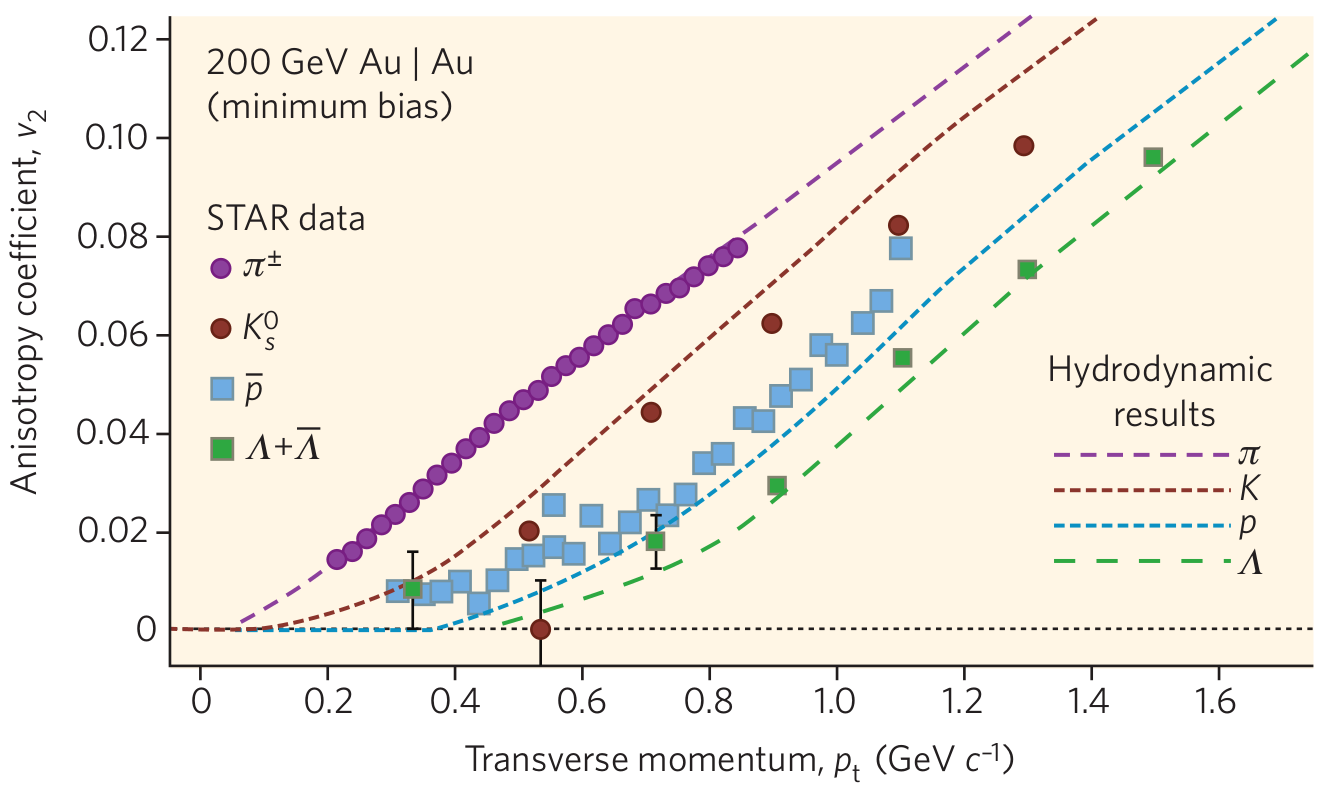
\includegraphics[width=0.9\textwidth]{Figures/Introduction/HeavyIons/RHICEllipticFlow.png}
 \caption{Elliptic flow distribution of as a function of transverse momentum for $\pi^{\pm}$ mesons, $K^{0}_{s}$ mesons, antiprotons and $\Lambda$ baryons measured by STAR collaboration in Au-Au collisions at $\sqrtsnn = \SI{200}{\GeV}$. The results are compared with relativistic hydrodynamic calculations. Figure taken from Ref.~\cite{RHICEllipticFlow}.}
 \label{fig:RHICEllipticFlow}
\end{figure}

At the start of the LHC, the CMS collaboration performed a measurement of the two-particle angular correlations in \Runpp collisions producing high number of particles (referred as high-multiplicity collisions). \fig{fig:CMSRidge} presents the two-particle $\Delta{\eta}$-$\Delta{\phi}$ correlation function measured by the CMS collaboration in \Runpp collisions at $\sqrts = \SI{7}{\TeV}$~\cite{CMSRidge}, where $\Delta{\phi}$ is the azimuthal angle difference between the two particles and $\Delta{\eta}$ is the difference in their pseudorapidity. The results show a long-range structure ($2.0 < \Delta{\eta} < 4.8$) of near-side ($\Delta{\phi} \sim 0$) two-particle  correlations, often called "ridge". The structure is seen for particles with $1~\GeVc < \pt < 3~\GeVc$, produced in high-multiplicity ($N > 110$) \Runpp collisions. A similar ridge-like structure had already been observed at RHIC in heavy-ion collisions~\cite{PHOBOSRidge}, which was understood as a result of the hydrodynamic expansion of the QGP, but the phenomenon found in \Runpp collisions was completely unexpected at the time and it is still not fully understood yet.

\begin{figure}[!htb]
 \centering
 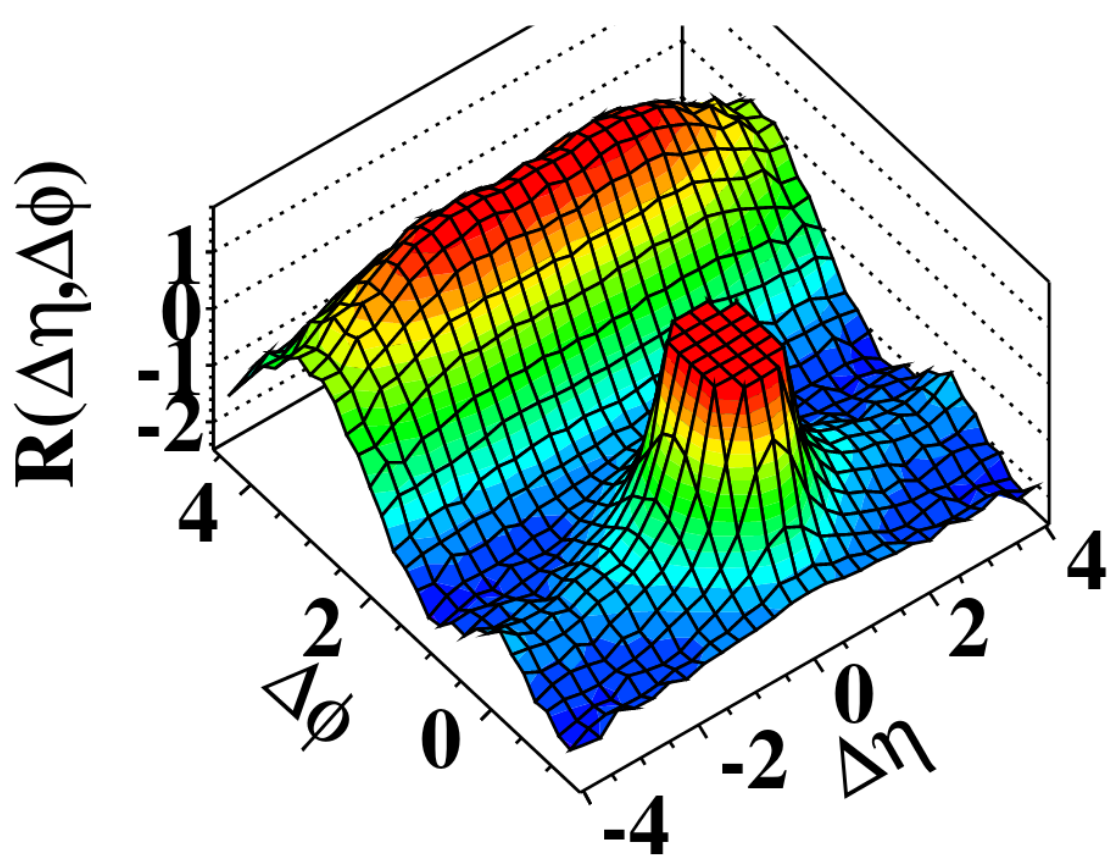
\includegraphics[width=0.6\textwidth]{Figures/Introduction/HeavyIons/Ridge.png}
 \caption{3D display of the $\Delta{\eta}$-$\Delta{\phi}$ correlation function between two charged particles with $1~\GeVc < \pt < 3~\GeVc$, measured by the CMS collaboration in high multiplicity ($N \geq 110$) \Runpp collisions at $\sqrts = \SI{7}{\TeV}$. Figure taken from Ref.~\cite{CMSRidge}.}
 \label{fig:CMSRidge}
\end{figure}


\subsubsection{Strangeness enhancement}

Strange quarks belongs to the second generation of quarks and are roughly 20-40 times more massive than up and down quarks. The number of strange quarks involved in a decay can be quantified through the quantum number called strangeness, which can take values of $+1$, $-1$ and 0, for strange quarks, strange anti-quarks, and the other quarks, respectively. Strangeness is conserved in strong and electromagnetic interactions, while it is not conserved in weak decays. In hadronic collisions, strange quark-antiquark pairs ($\cPqs\cPaqs$) are produced in parton-parton interactions via gluon fusion ($\cPg\cPg \rightarrow \cPqs\cPaqs$) or quark annihilation ($\cPq\cPaq \rightarrow \cPqs\cPaqs$), and through gluon splitting ($\cPg \rightarrow \cPqs\cPaqs$) during the evolution of the medium. The production of strange hadrons in proton-proton collisions is suppressed relative to hadrons made of light quarks (i.e. pions), due to the higher mass of the strange quark.

In heavy-ion collisions, where the QGP is formed, it was proposed by Johann Rafelski and Rolf Hagedorn~\cite{StrangenessEnhancement_1} in 1980, that the enhancement of strangeness could serve as a signature of the QGP. Due to the large gluon density and energy present in the hot medium, the gluon fusion becomes the dominant production mode of strange-quark pairs in the QGP. When the temperature of the QGP decreases and the partons hadronise, the production of hadrons containing strange (anti-)quarks is enhanced relative to the production of pions. Moreover, at high collision energies, the strange quarks can also bind to charm and bottom quarks during hadronisation, producing many exotic hadrons (e.g. strange $\D_{\cPqs}$ or $\B_{\cPqs}$ mesons) that would otherwise be rarely seen without the presence of the QGP. In summary, one expects an overall increase of strange-quark pair production, leading to an enhancement of the production of strange hadrons in central heavy-ion collisions compared to proton-proton collisions~\cite{StrangenessEnhancement_3}.

The enhancement of strange hadrons has been observed at SPS~\cite{SPS_StrangenessEnhancementExp_1,SPS_StrangenessEnhancementExp_2} and RHIC~\cite{StrangenessEnhancementExp_4}. The production yields in heavy-ion collisions of strange hadrons measured at RHIC and SPS are shown in \fig{fig:StrangenessEnhancementExp_1}. The results show a clear enhancement of the production of strange baryons in heavy-ion collisions relative to \Runpp (at RHIC) or p-Be (at SPS) collisions, increasing for higher \npart (more central collisions) and strangeness content ($\Omega^{-}$[sss] > $\Xi^{-}$[dss] > $\Lambda$[uds]). This strangeness enhancement can be described using a thermal model based on a grand canonical ensemble approach, suggesting the presence of a hot medium~\cite{StrangenessEnhancement_3}.

Recently, the ALICE collaboration published in~\cite{StrangenessEnhancementExp_3} the observation of enhanced production of strange hadrons in high-multiplicity proton-proton collisions at $\sqrts = \SI{7}{\TeV}$, as presented in the right plot of \fig{fig:StrangenessEnhancementExp_1}. The results at LHC show that the enhancement of the strangeness production increases as a function of charged-particle multiplicity from high-multiplicity p-p to p-Pb to Pb-Pb collisions. Therefore, further studies of the  mechanism of strangeness production at high multiplicities are necessary to understand the evolution of small systems.

\begin{figure}[!htb]
 \centering
 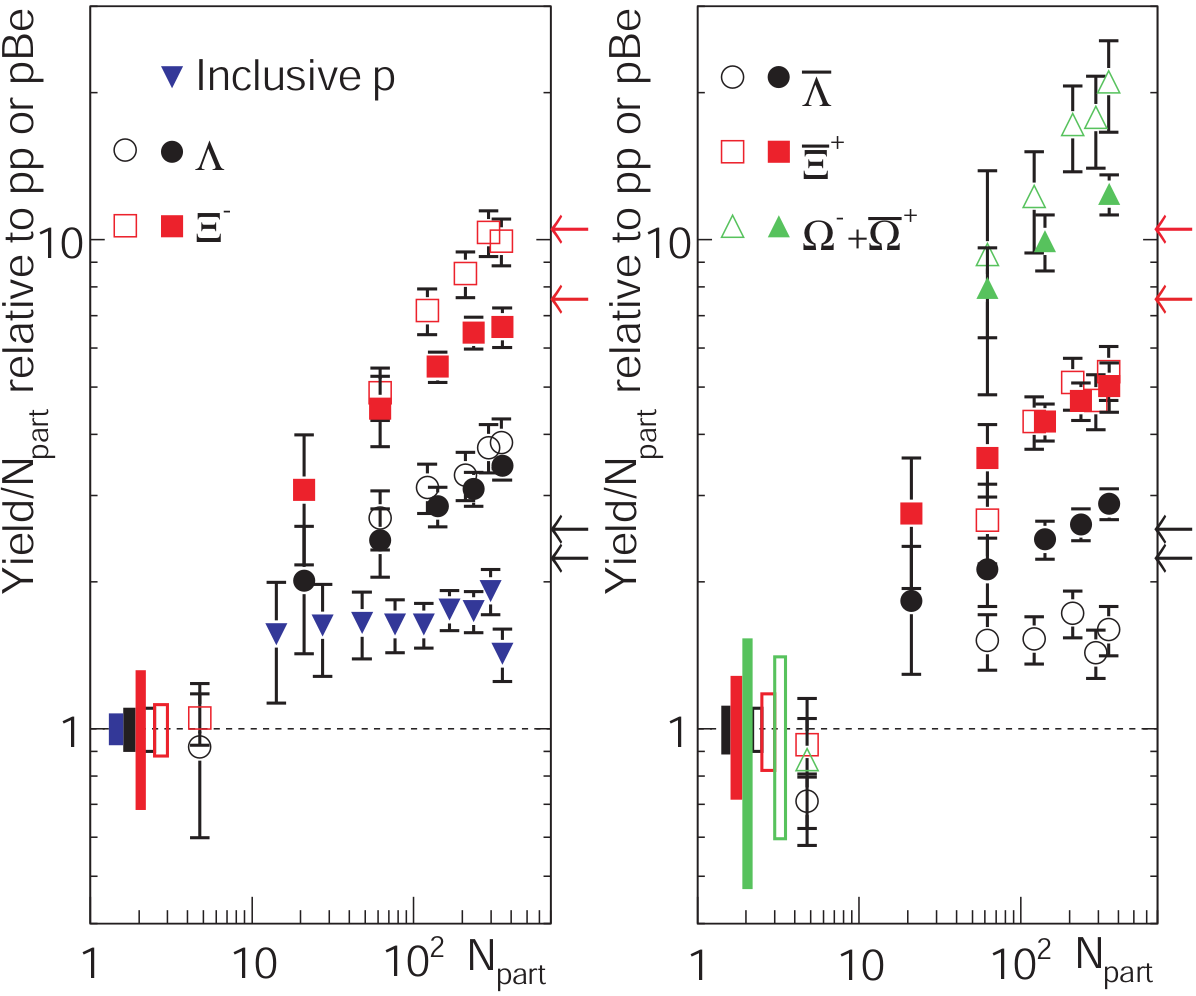
\includegraphics[width=0.56\textwidth]{Figures/Introduction/HeavyIons/SPS_RHIC_Strangeness.png}
 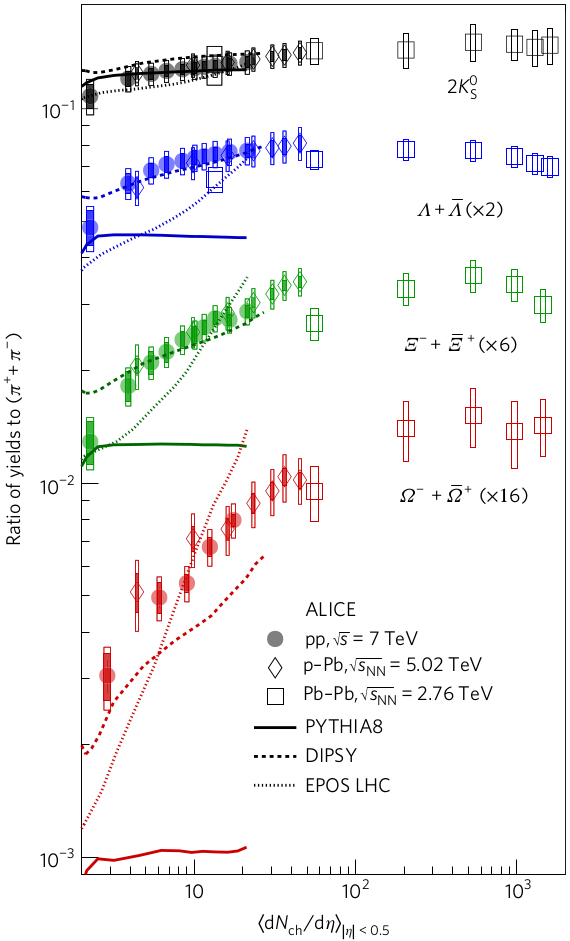
\includegraphics[width=0.42\textwidth]{Figures/Introduction/HeavyIons/ALICE_Strangeness.png}
 \caption{Left: Distribution of the yield of inclusive protons and strange baryons, measured by the STAR collaboration in Au-Au collisions at $\sqrtsnn = \SI{200}{\GeV}$ (solid symbols) and by the NA57 collaboration in \RunPbPb collisions at $\sqrtsnn = \SI{17.3}{\GeV}$ (empty symbols), relative to the corresponding yield in \Runpp (at RHIC) or p-Be (at SPS) collisions scaled by \npart. Figure from Ref.~\cite{StrangenessEnhancementExp_4}.
 Right: Distribution of the {\pt}-integrated yield ratios of strange hadrons to pions as a function of the average charged-particle multiplicity measured in $\abs{\eta} < 0.5$ by the ALICE collaboration in \Runpp, \RunpPb and \RunPbPb collisions at $\sqrts = \SI{7}{\TeV}$, $\sqrtsnn = \SI{5.02}{\TeV}$ and $\sqrtsnn = \SI{2.56}{\TeV}$, respectively. Figure from Ref.~\cite{StrangenessEnhancementExp_3}.}
 \label{fig:StrangenessEnhancementExp_1}
\end{figure}


\subsubsection{Jet quenching}\label{sec:Physics_HI_Probes_JetQuenching}

Energetic partons are produced in the hard scattering at the beginning of the collision. These scattered partons fragment into other colour-charged particles, which then create an ensemble of hadrons during the hadronisation process. The baryons and mesons produced at the end of the collision tend to move along the same direction as the original fragmented parton, forming a localised spray of particles called jet. The jets can be reconstructed by clustering hadrons and other particles around a given direction using a jet sequential recombination algorithm (e.g. anti-$k_{t}$~\cite{AntikT}).

In heavy-ion collisions, the hard partons lose energy when they traverse the hot medium either by multiple scattering with the medium constituents or by medium-induced gluon radiation. As a consequence, the energy of the jets is attenuated and the jets are considered quenched by the medium. The phenomenon of jet quenching in the QGP was first proposed in 1982 by James Bjorken. Bjorken suggested in~\cite{BjorkenJetQuenching} that the observation of events with two jets, where one of the jets escape the QGP without loosing energy while the other jet is fully quenched as shown in \fig{fig:JetQuenching}, could be used as a probe to determine the presence of the QGP.

\begin{figure}[!htb]
 \centering
 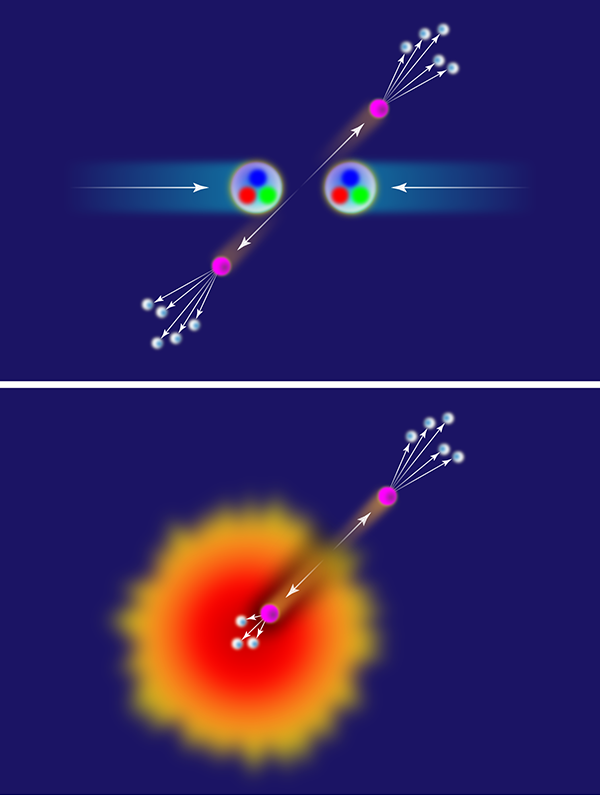
\includegraphics[width=0.4\textwidth]{Figures/Introduction/HeavyIons/JetQuenching.png}
 \caption{Sketch of the production mechanism of two jets in proton-proton (top) and heavy-ions (bottom) collisons. Figure taken from Ref.~\cite{FigureJetQuenching}.}
 \label{fig:JetQuenching}
\end{figure}

In order to quantify how the hot nuclear medium modifies the production of a given particle, one can measure the nuclear modification factor $R_{\text{AA}}$ defined as:

\begin{equation}
  R_{\text{AA}} = \frac{N_{\text{AA}}}{\left\langle\ncoll\right\rangle{N_{\text{pp}}}}
\end{equation}

where $N_{\text{AA}}$ is the yield of particles measured per nucleus-nucleus collision, $N_{\text{pp}}$ is the same yield measured per p-p collision, and $\left\langle\ncoll\right\rangle$ is the average number of binary nucleon-nucleon collisions. Proton-proton collisions are used as a reference since most of the events do not produce a QGP, even though it is not excluded that a hot medium could be formed in the most rare and violent \Runpp collisions.

The first direct observation of jet quenching was determined at RHIC, where the production of hadrons were found to be suppressed in central Au-Au collisions compared to \Runpp collisions. \fig{fig:RHICJetQuench} shows the nuclear modification factor of direct photons\footnote{Photons not originating from the decay of hadrons.}, pions, $\eta$ mesons, and charged hadrons measured at RHIC in central Au-Au collisions at $\sqrtsnn = \SI{200}{\GeV}$. The results show a strong suppression ($R_{\text{AA}} \sim 0.2$) of the production of hadrons consistent with parton energy loss in the QGP\footnote{At low \pt, extra thermal photons can be created by the medium providing insights on its average temperature~\cite{PHENIXPhoton}.}. In addition, the $R_{\text{AA}}$ of direct photons is found to be consistent with unity (expected since photons do not interact strongly), which serves as a sanity check of the \ncoll scaling.

\begin{figure}[!htb]
 \centering
 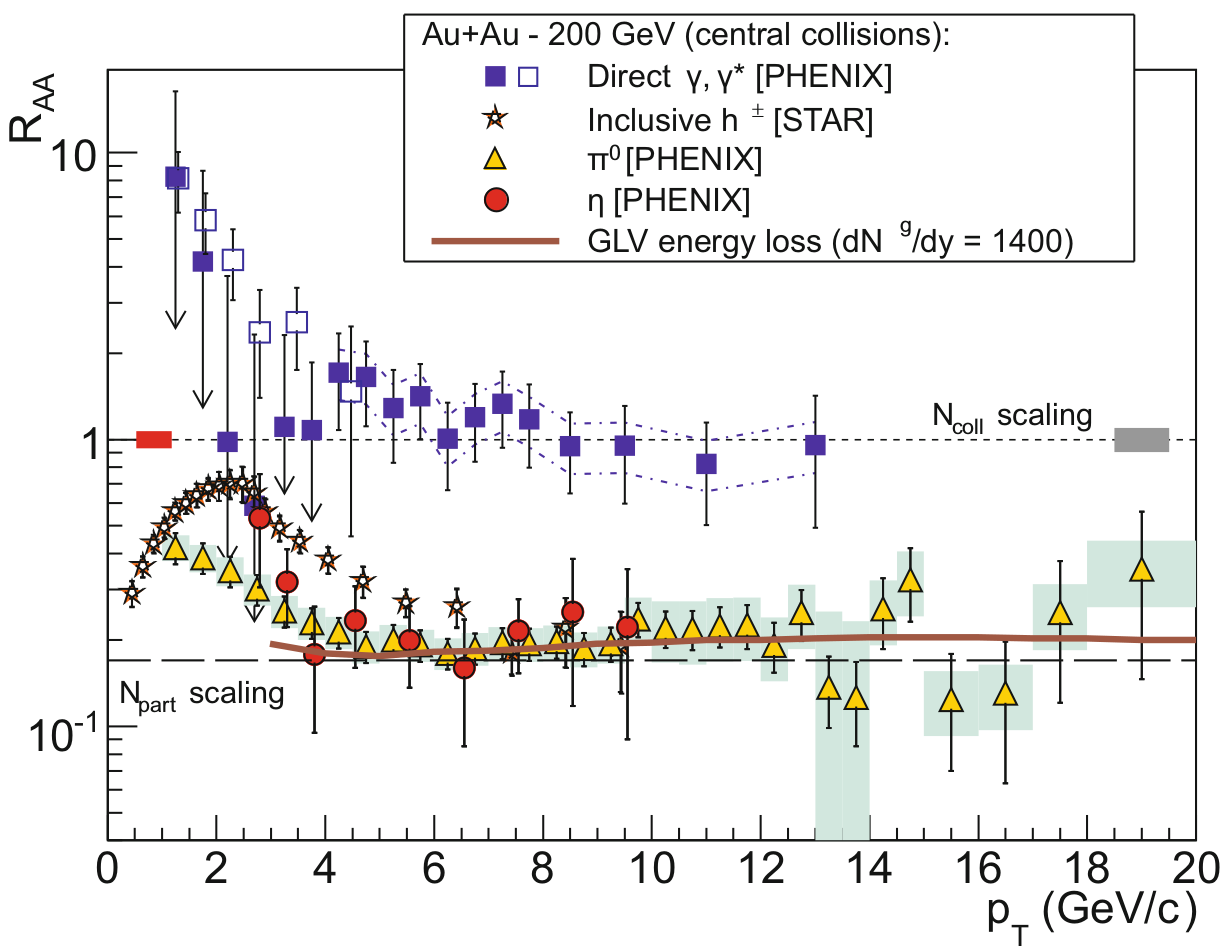
\includegraphics[width=0.7\textwidth]{Figures/Introduction/HeavyIons/PHENIXHadSupp.png}
 \caption{Distribution of the nuclear modification factor $R_{\text{AA}}$ of direct photons, pions, $\eta$ mesons and charged hadrons, measured at RHIC in central Au-Au collisions at $\sqrtsnn = \SI{200}{\GeV}$. Theoretical predictions of radiative parton energy loss are also included. Figure taken from Ref.~\cite{RHICJetQuench}.}
 \label{fig:RHICJetQuench}
\end{figure}

In the case of LHC, an enhanced dijet asymmetry was observed in Pb-Pb collisions compared to proton-proton collisions. The dijet asymmetry is quantified by measuring the jet energy imbalance between the two highest transverse energy jets with an azimuthal angle separation of ${\Delta}{\phi} = |\phi_{1} - \phi_{2}| > {\pi}/{2}$. The jet energy imbalance $A_{J}$ is derived as:

\begin{equation}
  A_{J} = \frac{E_{T1} - E_{T2}}{E_{T1} + E_{T2}}
\end{equation}

where $E_{T1}$ is the transverse energy of the most energetic jet among the pair of jets. \ref{fig:ATLASDijetAsym} presents the results, published by the ATLAS collaboration~\cite{ATLASDijetAsym}, of the dijet asymmetry distribution and the azimuthal angle between the two jets in different bins of centrality. The dijet asymmetry measured in Pb-Pb collisions at $\sqrtsnn = 2.76$~TeV are compared to the measurements from p-p collisions at $\sqrts = \SI{7}{\TeV}$ and the simulated results derived using events from the Heavy Ion Jet INteraction Generator (\HIJING) superimposed with \PYTHIA events. The LHC results show a significant dijet energy imbalance in Pb-Pb collisions which increases with the centrality of the collision. The missing jet energy was later found in the form of low-momentum particles emitted at larger angles~\cite{CMSDijetAsym}. This dijet asymmetry is not seen in p-p collisions evidencing the strong jet energy loss present in the QGP.

\begin{figure}[!htb]
 \centering
 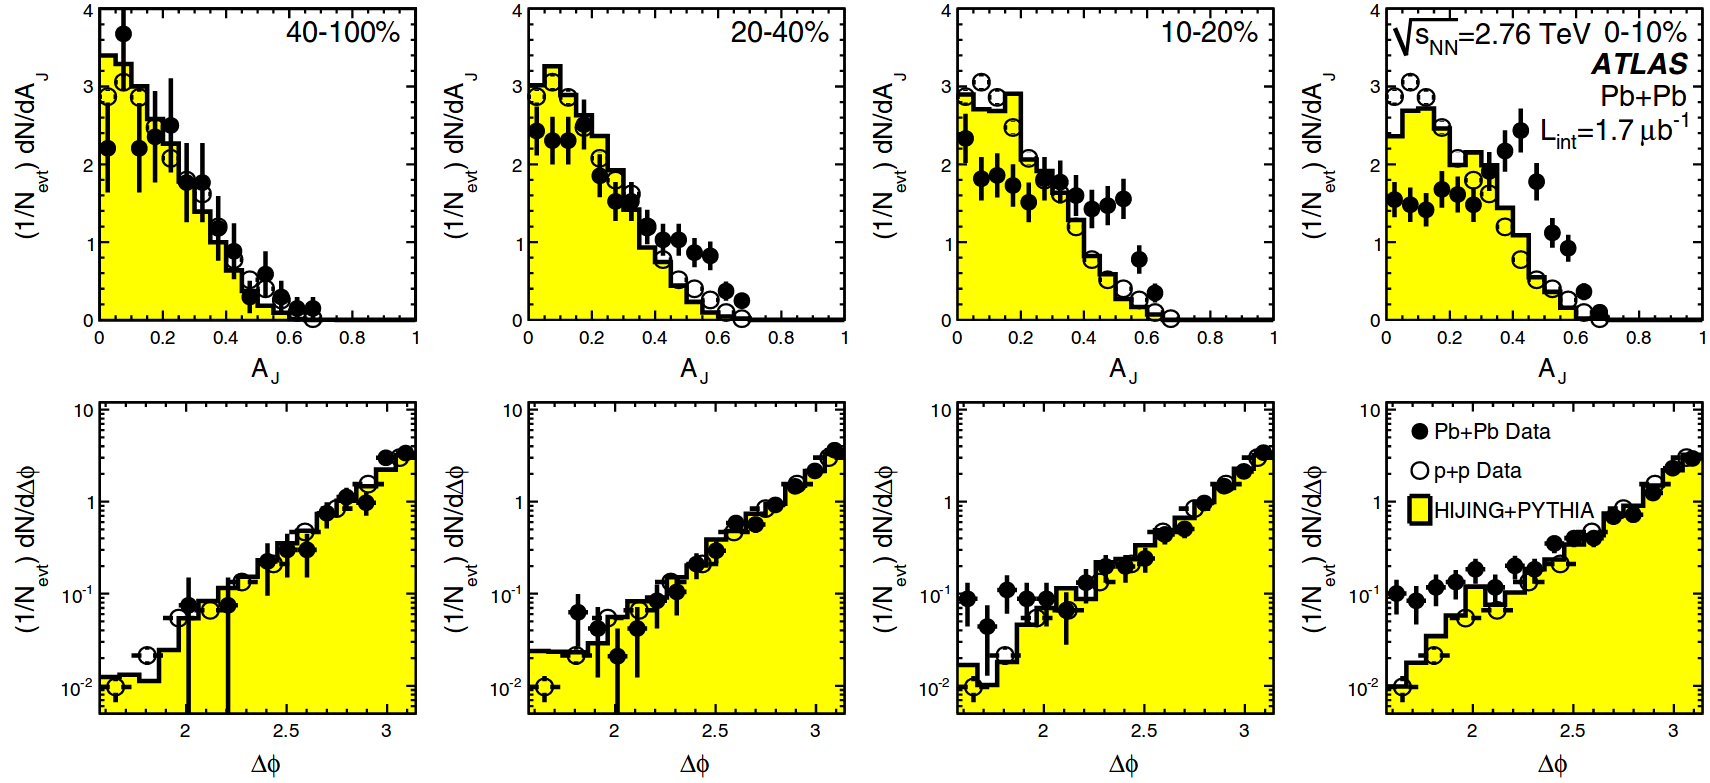
\includegraphics[width=1.0\textwidth]{Figures/Introduction/HeavyIons/ATLASDijetAsym.png}
 \caption{Dijet asymmetry measured by the ATLAS collaboration in lead-lead collisions at $\sqrtsnn = 2.76$~TeV (points) and proton-proton collisions at $\sqrts=7$~TeV (open circles). The top panel shows the dijet asymmetry distributions and unquenched \HIJING with superimposed \PYTHIA dijets (solid yellow histograms), as a function of collision centrality. The bottom panel shows the distribution of the azimuthal angle between the two jets ${\Delta}{\phi}$, for data and {\HIJING}+{\PYTHIA}, also as a function of centrality. Figure taken from Ref.~\cite{ATLASDijetAsym}.}
 \label{fig:ATLASDijetAsym}
\end{figure}


\subsubsection{Quarkonium production}\label{sec:Physics_HI_Probes_Quarkonium}

Quarkonia (\QQbar) are mesons composed of a heavy quark and its own anti-quark. Quarkonia can be classified as charmonia or bottomonia if they are made of charm quarks or bottom quarks, respectively. The first excited state of charmonia is called \JPsi meson while for bottomonia is called \UpsOneS meson. The properties of quarkonia are non-perturbative but since the mass of the heavy quarks is comparable to the mass of the quarkonia, the quarks move inside the quarkonia much slower than the speed of light. As a result, the properties of quarkonia can be computed using an effective non-relativistic model. For instance, one way to describe the binding of the quarks is by using a Cornell potential~\cite{QuarkoniumPotential} given by:

\begin{equation}
 V_{\QQbar}\left(r\right) = -\frac{a}{r} + br
 \label{eq:QQbar}
\end{equation}

where $r$ is the binding radius of the quarkonium, $a$ is the coulombic interaction coupling, and $b$ is the string tension. By solving the Schr{\"o}dinger equation for the \QQbar potential, one finds several higher excited states of charmonia (e.g. \PsiP) and bottomonia (e.g. \UpsTwoS and \UpsThreeS), with lower binding energies and larger radius (i.e. $r_{\UpsOneS} < r_{\UpsTwoS} < r_{\UpsThreeS}$).

One of the first signatures suggested to probe the QGP was the suppression of \JPsi meson production. In 1986, Tetsuo Matsui and Helmut Satz~\cite{JpsiSuppression} proposed that the \JPsi meson binding potential gets screened in the QGP due to the interactions with the free colour charged constituents of the hot medium. The Debye colour screening potential increases with the temperature of the medium until the binding potential can no longer hold the quarks together, and the quarkonium "melts". The binding potential of quarkonium states gets weaker for larger binding radius. As a result, the higher excited states of quarkonium are expected to be more dissociated at a given temperature compared to the ground state, leading to a sequential suppression of quarkonia.

The sequential suppression of bottomonium states has been observed at the LHC. Figure~\ref{fig:CMSUpsilonSuppression} shows the invariant mass distribution of dimuons measured by the CMS collaboration in Pb-Pb collisions at $\sqrtsnn = \SI{5.02}{\TeV}$~\cite{CMSUpsilonSuppression}. The result is compared to the invariant mass distribution obtained by adding the bottomonium mass peaks extracted from \Runpp collisions at $\sqrts = 5.02$~TeV on top of the \RunPbPb background and normalised to the \UpsOneS mass peak in \RunPbPb. The comparison shows a clear suppression pattern where the \UpsThreeS meson is completely melted while part of the \UpsTwoS mass peak still survives. In the case of the \UpsOneS meson, the feed-down contributions from excited state decays of $\chi_{b}(\text{nP}))\rightarrow\UpsOneS$ and $\upsilon(\text{nS})\rightarrow\UpsOneS$, can reach values up to 40\% as measured by the LHCb collaboration for $\pt^{\Upsilon} > 6~\GeVc$~\cite{LHCbFeedDownUpsOneS}. As a result, it is not clear if the observed suppression of the \UpsOneS meson is due to deconfinement in the QGP or the dissociation of the excited states that decays to the \UpsOneS meson.

\begin{figure}[!htb]
 \centering
 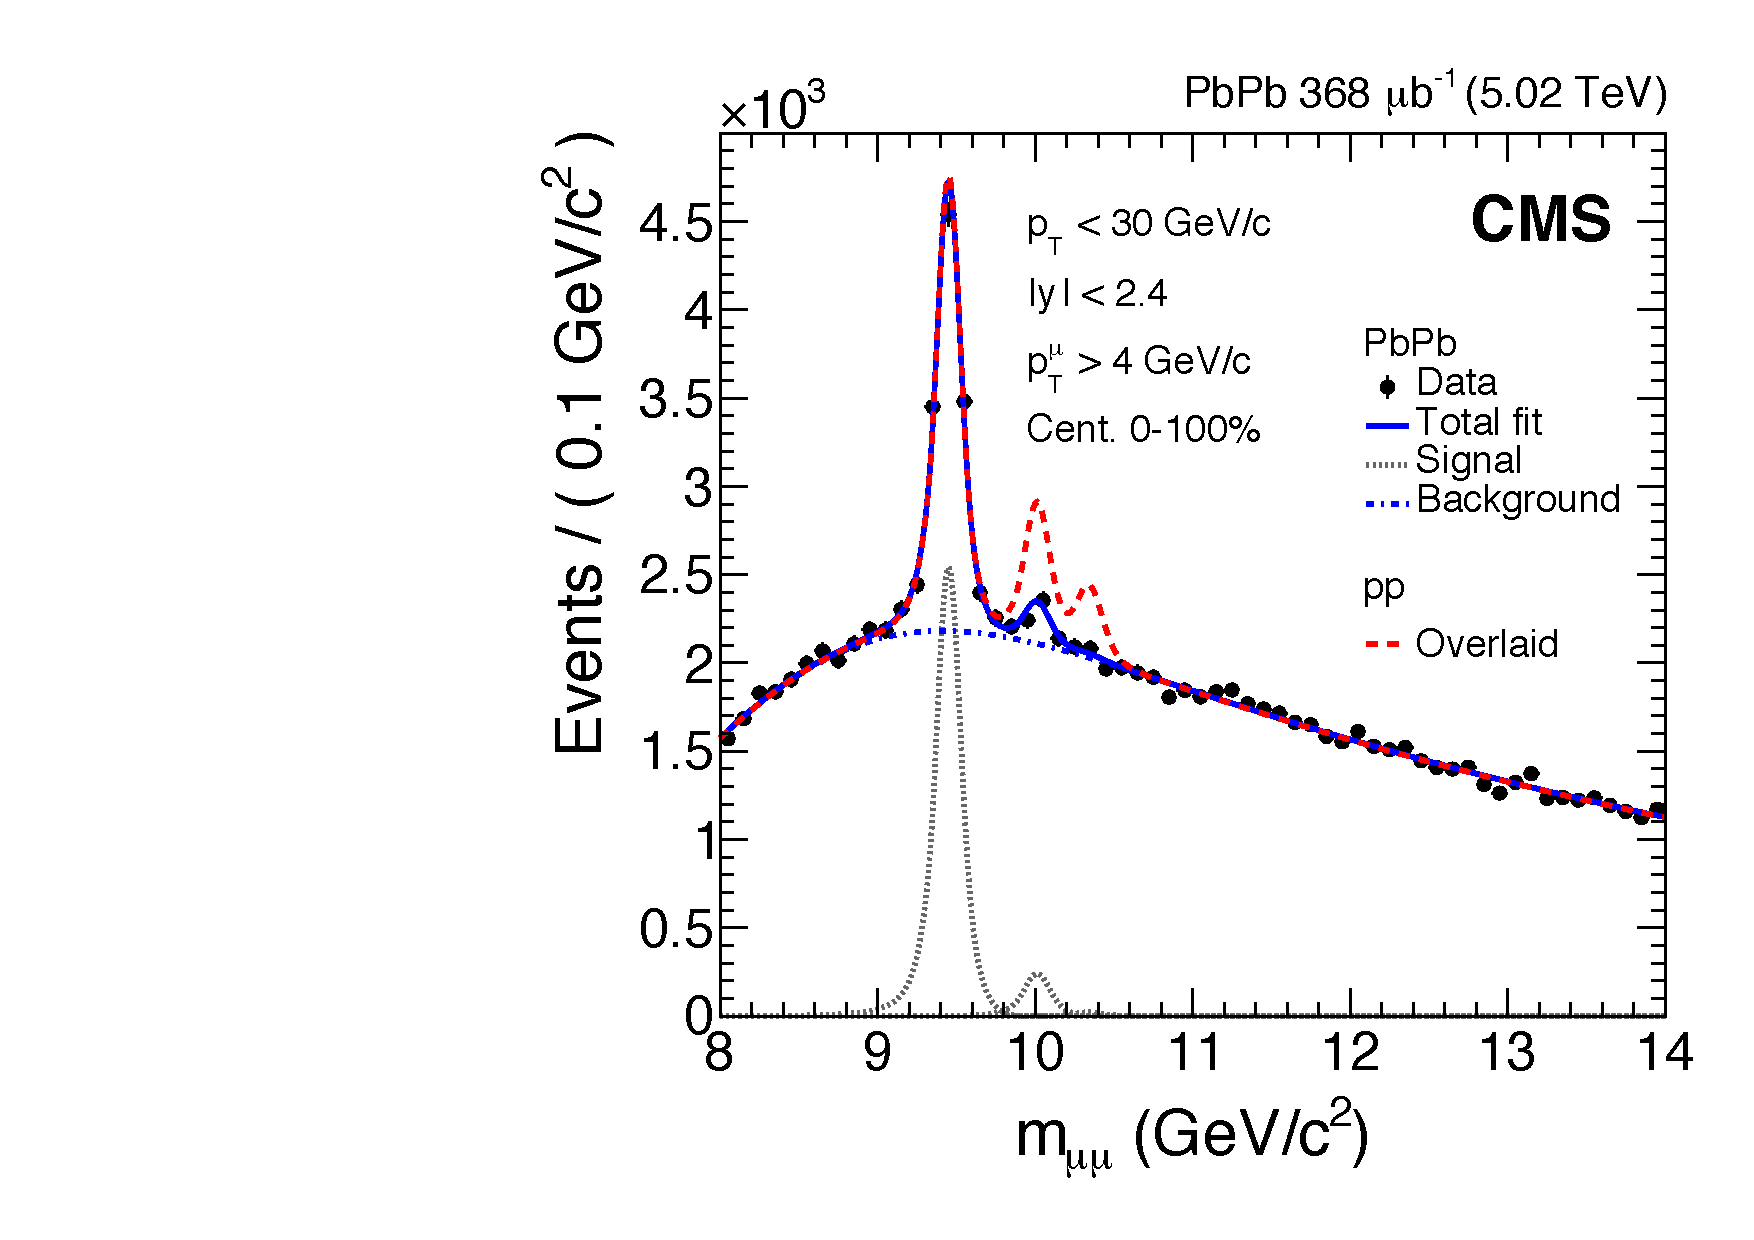
\includegraphics[width=0.6\textwidth]{Figures/Introduction/HeavyIons/UpsilonSuppression.pdf}
 \caption{Dimuon invariant mass distribution measured by the CMS collaboration in Pb-Pb collisions at $\sqrtsnn = 5.02$~TeV. The total fit (solid blue line), the background component (dot-dashed blue line) and the individual \UpsOneS, \UpsTwoS and \UpsThreeS mass peaks (dotted gray lines) are shown. The dashed red line represents the p-p signal shapes added on top of the Pb-Pb background and normalised to the \UpsOneS mass peak in Pb-Pb. Figure taken from Ref.~\cite{CMSUpsilonSuppression}.}
 \label{fig:CMSUpsilonSuppression}
\end{figure}

The first evidence of \JPsi-meson anomalous suppression (i.e. beyond nuclear effects) was observed in \RunPbPb collisions at \SI{158}{\GeV}/nucleon by the NA50 collaboration at SPS~\cite{SPSJpsiSuppression_1}. The results at SPS showed that the \JPsi-meson cross section measured in peripheral collisions was consistent with the expectations from nuclear absorption while in central collisions it was more suppressed~\cite{SPSJpsiSuppression_2}. The measurement of the \JPsi-meson production in Au-Au collisions at $\sqrtsnn = \SI{200}{\GeV}$ at RHIC~\cite{JpsiRHIC} showed a similar level of suppression at mid-rapidity ($\abs{y} < 0.35$) compared to SPS, despite the higher energy density at RHIC. In addition, the production of \JPsi mesons at forward rapidity ($1.2 < \abs{y} < 2.2$) was found to be more suppressed than at mid-rapidity.

To understand the measurements of \JPsi-meson production at SPS and RHIC, two explanations were proposed. The first one suggested that, apart from the anomalous suppression, the \JPsi meson production could also be enhanced at RHIC energies. According to~\cite{JpsiRegeneration}, the \JPsi mesons could be regenerated in the most central collisions from the combination of initially uncorrelated charm quarks (i.e. not produced in the same hard scattering). The number of directly produced \ccbar pairs in central nucleus-nucleus collisions is expected to be small at SPS energies, but it can reach values around 10 (200) charm-quark pairs at RHIC (LHC) energies~\cite{UncorrelatedCharms,UncorrelatedCharms_2}. The second explanation proposed that the production of \JPsi mesons at RHIC was mainly affected by an interplay between initial state effects (e.g. nuclear PDFs or CGC) and the dissociation of the excited states (e.g. $\chi_{c}$ and \PsiP) that contributes to the feed-down of the \JPsi meson.

The measurements of the \JPsi-meson production have also been performed at the LHC. The results of the \JPsi-meson nuclear modification factor measured by the ALICE collaboration in the $0\%-20\%$ most central Pb-Pb collisions at $\sqrtsnn = \SI{2.76}{\TeV}$ are compared in \fig{fig:ALICEJpsiRegeneration} to the results measured by the PHENIX collaboration in the $0\%-20\%$ most central Au-Au collisions at $\sqrtsnn = \SI{200}{\GeV}$. The \JPsi $R_{AA}$ measured at the LHC is larger than the one measured at RHIC at low \JPsi meson \pt, which can so far only be explained by the presence of regeneration.

\begin{figure}[!htb]
 \centering
 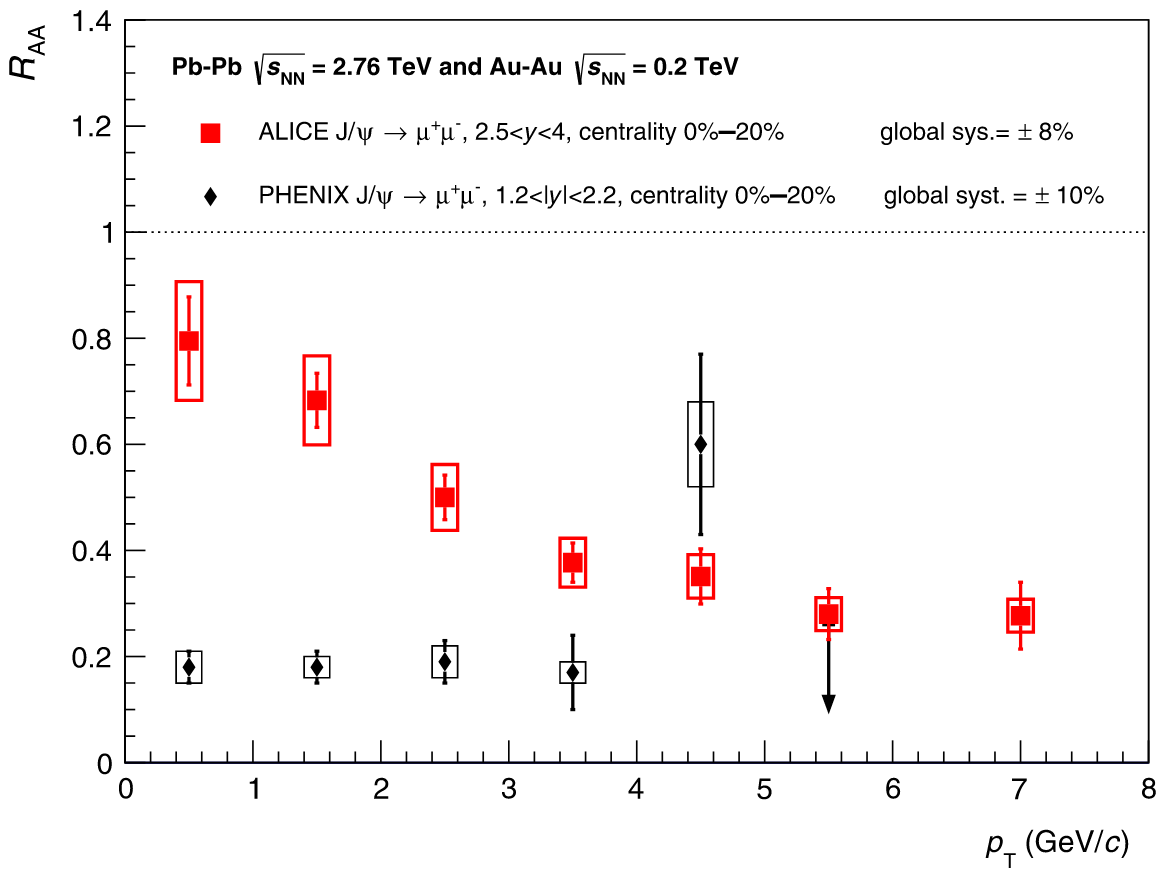
\includegraphics[width=0.6\textwidth]{Figures/Introduction/HeavyIons/JpsiRegeneration.png}
 \caption{Nuclear modification factor of \JPsi meson as a function of transverse momentum measured by the ALICE collaboration in the $0\%-20\%$ most central Pb-Pb collisions at $\sqrtsnn = 2.76$~TeV compared to results from the PHENIX collaboration measured in the $0\%-20\%$ most central Au-Au collisions at $\sqrtsnn = 200$~GeV. Figure taken from Ref.~\cite{ALICEJpsiRegeneration}.}
 \label{fig:ALICEJpsiRegeneration}
\end{figure}


\subsubsection{Electroweak boson production}

Electroweak particles, such as {\PW} bosons and {\PZ} bosons, are produced in the parton-parton hard scattering and they do not interact strongly with the nuclear medium produced in the heavy-ion  collisions. As a result, electroweak bosons are good probes of the initial stage of the proton-nucleus (p-A) and nucleus-nucleus (A-A) collisions, but they do not probe the QGP. The dominant production mode of electroweak bosons in heavy-ion collisions is via the annihilation of a light quark and anti-quark. The large momentum scales involved in the production of weak bosons allows to derive precise calculations of their partonic cross sections using pQCD.

The production yields of electroweak bosons in p-A or A-A collisions are affected by the mix of protons and neutrons in the colliding nucleus (isospin effect), and the depletion (shadowing) or enhancement (anti-shadowing) of the PDFs in the nucleus. Thus, the measurement of the electroweak boson production in heavy-ion collisions can be used to set constrains to the global fits of the nuclear PDFs. In the case of A-A collisions, the measurement of the nuclear modification factor of \Z bosons at the LHC in Pb-Pb collisions at $\sqrtsnn = 2.56$~TeV~\cite{CMSZBosonPbPb}, presented in \fig{fig:CMSZBosonPbPb}, shows that the production of weak bosons is not modified by the hot nuclear medium and can then be used as a \textit{standard candle} to check, at first order, the binary scaling ($R_{\text{AA}} = 1$) and indirectly determine the centrality of the collision.

\begin{figure}[!htb]
 \centering
 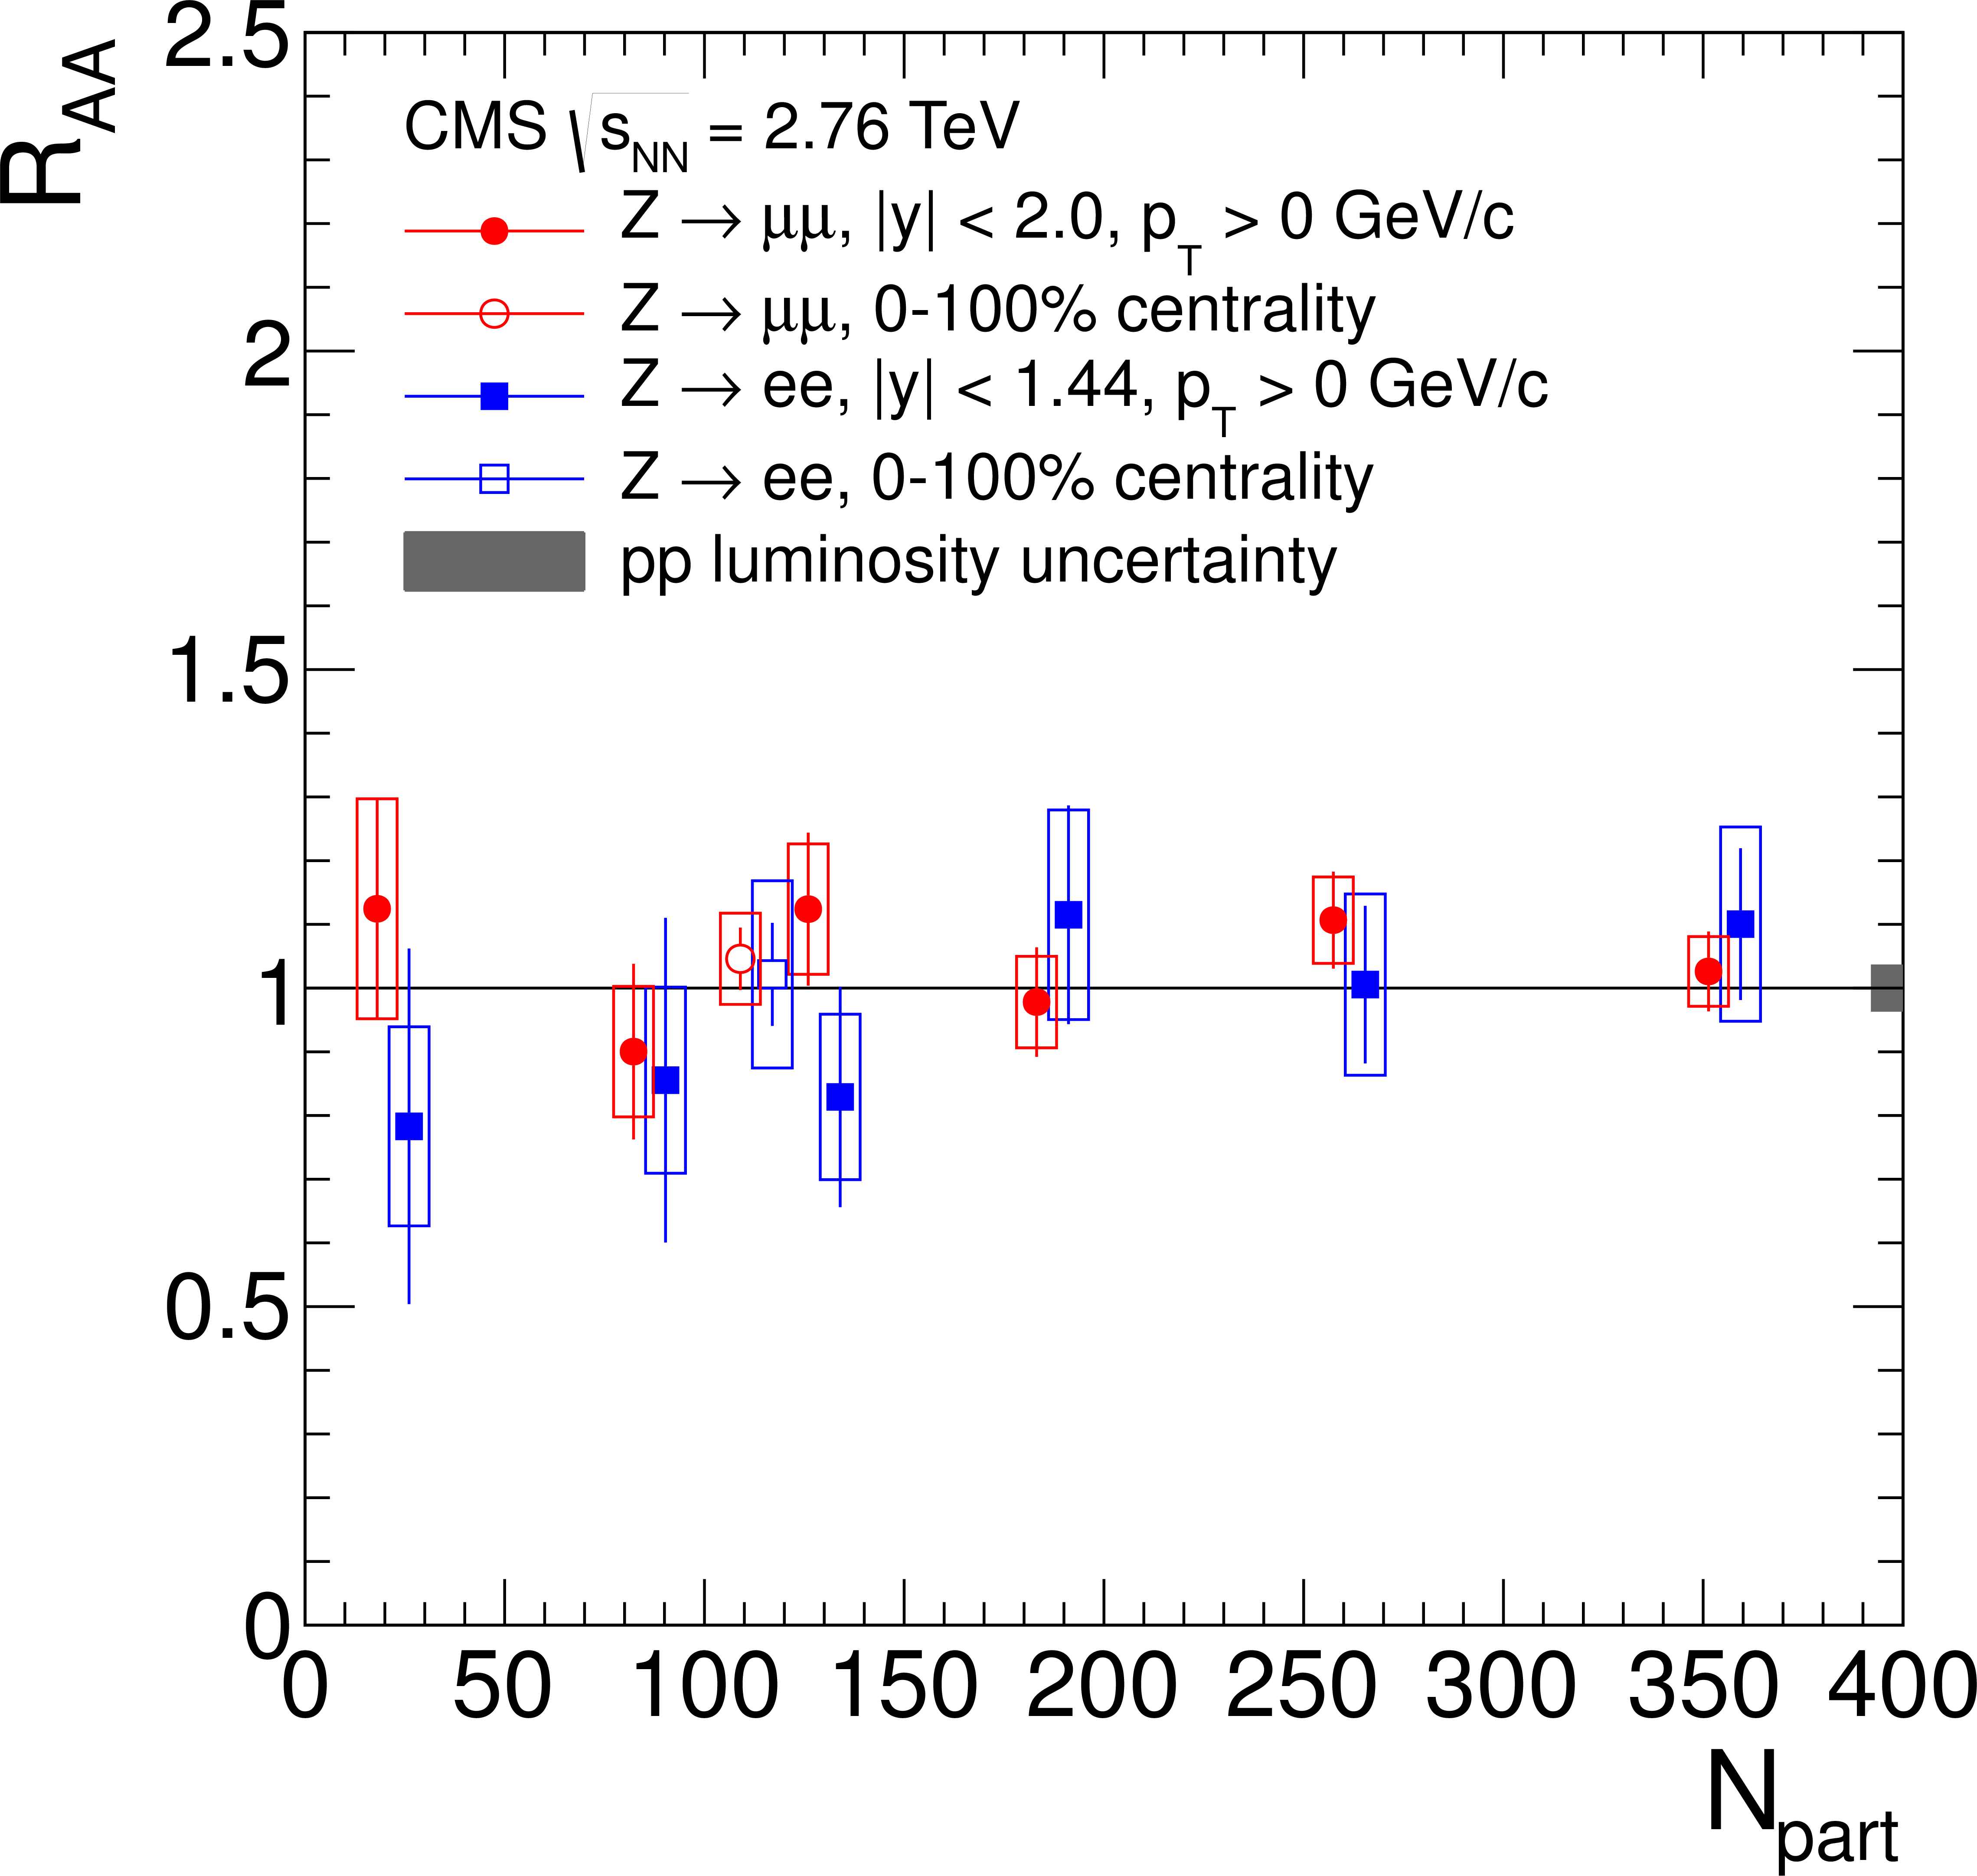
\includegraphics[width=0.55\textwidth]{Figures/Introduction/HeavyIons/CMSZBosonPbPb.png}
 \caption{Nuclear modification factor $R_{\text{AA}}$ of $\Z \rightarrow e^{+}e^{-}$ (blue squares) and $\ZToMuMu$ (red circles) events as a function of \npart measured by the CMS collaboration in \RunPbPb collisions at $\sqrtsnn = \SI{2.56}{\TeV}$. The open points represent the centrality-integrated $R_{\text{AA}}$ and the vertical lines (boxes) correspond to statistical (systematic) uncertainties. Figure taken from Ref.~\cite{CMSZBosonPbPb}.}
 \label{fig:CMSZBosonPbPb}
\end{figure}


\section*{Summary}\label{sec:Physics_Summary}

Our understanding of the QGP has expanded substantially since the last 20 years. The first evidence of its existence was found at SPS, after studying the suppression of \JPsi mesons and the strangeness enhancement in \RunPbPb collisions. Years after, the first observation of the QGP was claimed at RHIC, supported by a vast amount of experimental signatures such as jet quenching, charmonium suppression, strangeness enhancement and  collectivity. The QGP found at RHIC turns out to behave as a nearly perfect dense fluid. The QGP was later also observed at the LHC, which has provided further knowledge on the properties of the QGP at TeV energies. In addition, the LHC experiments have also observed hints of the formation of a collective medium in small systems such as high-multiplicity \Runpp collisions, which is still not fully understood.

The production of \JPsi mesons in heavy-ion collisions has shown a rich phenomenology and will be the main topic of \chp{sec:Charmonia}, where the analysis of charmonia in \RunPbPb collisions will be presented. These results provide new insights on the production of non-prompt \JPsi mesons (i.e. from b-hadron decays) and \PsiP mesons, extending the coverage to higher charmonium \pt ranges.

Electroweak bosons are sensitive probes of the initial state of the collision and the measurement of their production in heavy-ion collisions can be used to constrain the nuclear PDFs, which are crucial theoretical inputs for a better description of the formation of the QGP. In \chp{sec:WBoson}, this thesis reports the fist  measurement of significant nuclear modification of \Wb-boson production.

% END OF SECTION


% END OF CHAPTER
\clearpage
